% Options for packages loaded elsewhere
% Options for packages loaded elsewhere
\PassOptionsToPackage{unicode}{hyperref}
\PassOptionsToPackage{hyphens}{url}
\PassOptionsToPackage{dvipsnames,svgnames,x11names}{xcolor}
%
\documentclass[
  letterpaper,
  DIV=11,
  numbers=noendperiod,
  oneside]{scrreprt}
\usepackage{xcolor}
\usepackage[left=1in,marginparwidth=2.0666666666667in,textwidth=4.1333333333333in,marginparsep=0.3in]{geometry}
\usepackage{amsmath,amssymb}
\setcounter{secnumdepth}{5}
\usepackage{iftex}
\ifPDFTeX
  \usepackage[T1]{fontenc}
  \usepackage[utf8]{inputenc}
  \usepackage{textcomp} % provide euro and other symbols
\else % if luatex or xetex
  \usepackage{unicode-math} % this also loads fontspec
  \defaultfontfeatures{Scale=MatchLowercase}
  \defaultfontfeatures[\rmfamily]{Ligatures=TeX,Scale=1}
\fi
\usepackage{lmodern}
\ifPDFTeX\else
  % xetex/luatex font selection
\fi
% Use upquote if available, for straight quotes in verbatim environments
\IfFileExists{upquote.sty}{\usepackage{upquote}}{}
\IfFileExists{microtype.sty}{% use microtype if available
  \usepackage[]{microtype}
  \UseMicrotypeSet[protrusion]{basicmath} % disable protrusion for tt fonts
}{}
\makeatletter
\@ifundefined{KOMAClassName}{% if non-KOMA class
  \IfFileExists{parskip.sty}{%
    \usepackage{parskip}
  }{% else
    \setlength{\parindent}{0pt}
    \setlength{\parskip}{6pt plus 2pt minus 1pt}}
}{% if KOMA class
  \KOMAoptions{parskip=half}}
\makeatother
% Make \paragraph and \subparagraph free-standing
\makeatletter
\ifx\paragraph\undefined\else
  \let\oldparagraph\paragraph
  \renewcommand{\paragraph}{
    \@ifstar
      \xxxParagraphStar
      \xxxParagraphNoStar
  }
  \newcommand{\xxxParagraphStar}[1]{\oldparagraph*{#1}\mbox{}}
  \newcommand{\xxxParagraphNoStar}[1]{\oldparagraph{#1}\mbox{}}
\fi
\ifx\subparagraph\undefined\else
  \let\oldsubparagraph\subparagraph
  \renewcommand{\subparagraph}{
    \@ifstar
      \xxxSubParagraphStar
      \xxxSubParagraphNoStar
  }
  \newcommand{\xxxSubParagraphStar}[1]{\oldsubparagraph*{#1}\mbox{}}
  \newcommand{\xxxSubParagraphNoStar}[1]{\oldsubparagraph{#1}\mbox{}}
\fi
\makeatother


\usepackage{longtable,booktabs,array}
\usepackage{calc} % for calculating minipage widths
% Correct order of tables after \paragraph or \subparagraph
\usepackage{etoolbox}
\makeatletter
\patchcmd\longtable{\par}{\if@noskipsec\mbox{}\fi\par}{}{}
\makeatother
% Allow footnotes in longtable head/foot
\IfFileExists{footnotehyper.sty}{\usepackage{footnotehyper}}{\usepackage{footnote}}
\makesavenoteenv{longtable}
\usepackage{graphicx}
\makeatletter
\newsavebox\pandoc@box
\newcommand*\pandocbounded[1]{% scales image to fit in text height/width
  \sbox\pandoc@box{#1}%
  \Gscale@div\@tempa{\textheight}{\dimexpr\ht\pandoc@box+\dp\pandoc@box\relax}%
  \Gscale@div\@tempb{\linewidth}{\wd\pandoc@box}%
  \ifdim\@tempb\p@<\@tempa\p@\let\@tempa\@tempb\fi% select the smaller of both
  \ifdim\@tempa\p@<\p@\scalebox{\@tempa}{\usebox\pandoc@box}%
  \else\usebox{\pandoc@box}%
  \fi%
}
% Set default figure placement to htbp
\def\fps@figure{htbp}
\makeatother





\setlength{\emergencystretch}{3em} % prevent overfull lines

\providecommand{\tightlist}{%
  \setlength{\itemsep}{0pt}\setlength{\parskip}{0pt}}



 


\KOMAoption{captions}{tableheading}
\makeatletter
\@ifpackageloaded{bookmark}{}{\usepackage{bookmark}}
\makeatother
\makeatletter
\@ifpackageloaded{caption}{}{\usepackage{caption}}
\AtBeginDocument{%
\ifdefined\contentsname
  \renewcommand*\contentsname{Table of contents}
\else
  \newcommand\contentsname{Table of contents}
\fi
\ifdefined\listfigurename
  \renewcommand*\listfigurename{List of Figures}
\else
  \newcommand\listfigurename{List of Figures}
\fi
\ifdefined\listtablename
  \renewcommand*\listtablename{List of Tables}
\else
  \newcommand\listtablename{List of Tables}
\fi
\ifdefined\figurename
  \renewcommand*\figurename{Figure}
\else
  \newcommand\figurename{Figure}
\fi
\ifdefined\tablename
  \renewcommand*\tablename{Table}
\else
  \newcommand\tablename{Table}
\fi
}
\@ifpackageloaded{float}{}{\usepackage{float}}
\floatstyle{ruled}
\@ifundefined{c@chapter}{\newfloat{codelisting}{h}{lop}}{\newfloat{codelisting}{h}{lop}[chapter]}
\floatname{codelisting}{Listing}
\newcommand*\listoflistings{\listof{codelisting}{List of Listings}}
\makeatother
\makeatletter
\makeatother
\makeatletter
\@ifpackageloaded{caption}{}{\usepackage{caption}}
\@ifpackageloaded{subcaption}{}{\usepackage{subcaption}}
\makeatother
\makeatletter
\@ifpackageloaded{sidenotes}{}{\usepackage{sidenotes}}
\@ifpackageloaded{marginnote}{}{\usepackage{marginnote}}
\makeatother
\usepackage{bookmark}
\IfFileExists{xurl.sty}{\usepackage{xurl}}{} % add URL line breaks if available
\urlstyle{same}
\hypersetup{
  pdftitle={EE6653 - Power Electronics Notes},
  pdfauthor={Qiaoxuan Zhang},
  colorlinks=true,
  linkcolor={blue},
  filecolor={Maroon},
  citecolor={Blue},
  urlcolor={Blue},
  pdfcreator={LaTeX via pandoc}}


\title{EE6653 - Power Electronics Notes}
\author{Qiaoxuan Zhang}
\date{2026-05-06}
\begin{document}
\maketitle

\renewcommand*\contentsname{Table of contents}
{
\hypersetup{linkcolor=}
\setcounter{tocdepth}{2}
\tableofcontents
}

\bookmarksetup{startatroot}

\chapter*{Preface}\label{preface}
\addcontentsline{toc}{chapter}{Preface}

\markboth{Preface}{Preface}

This is the course notes for EE6653: Power Electronics taught by
Prof.~Shuang Xu at the University of New Brunswick in Summer 2026.

\[
\textbf{Interdisciplinary course} \quad \begin{cases}
\underline{\text{Electronics}}\\
\underline{\text{Electric circuits}}\\
\underline{\underline{\text{Control}}} \qquad \begin{array}{rl}\small\searrow \hspace{-2ex}&\tiny{\text{AC--AC converters}}\\[-2ex]&\tiny{\text{Resonance converters}}\end{array}
\end{cases}
\]

\textbf{Course objective}:

Solidify your basic knowledge.

\bookmarksetup{startatroot}

\chapter{Convolution}\label{convolution}

\section{Linear Time-Invariant (LTI)
Systems}\label{linear-time-invariant-lti-systems}

\pandocbounded{\includegraphics[keepaspectratio]{index_files/mediabag/f782e5f1ee378178f14a4d44f892467e45d9f744.pdf}}

~ Classical control theory (root locus, Bode plot)

\subsection*{3 properties}\label{properties}
\addcontentsline{toc}{subsection}{3 properties}

\(\color{RedOrange}\boxed{\textbf{Homogeneity}}\)

\begin{figure}

\begin{minipage}{0.50\linewidth}
\begin{equation}
\underset{\quad\quad\quad \color{magenta} {}^{\uparrow_{\hspace{-3pt}\_\_\_}}\,\,\text{scaling factor}}
{\begin{array}{rcl}
\text{if} \quad x & \rightarrow & y \\
\text{then} \quad 2x & \rightarrow & 2y \\
\color{magenta}a \color{black} \,x & \rightarrow & \color{magenta}a \color{black} \,y
\end{array}}
\end{equation}\end{minipage}%
%
\begin{minipage}{0.50\linewidth}

\begin{array}{rcll}
\color{ForestGreen} \text{E.g.}\quad\text{Is}\quad y & \color{ForestGreen} = & \color{ForestGreen} 3x+1 & \color{ForestGreen} \text{LTI ?} \\
\color{blue} 4 & & \color{blue} 1 & \\
\color{blue} 7 & & \color{blue} 2 & \color{Magenta}\text{NO} \\
\color{blue} 10 & & \color{blue} 3 & \\[2ex]
\color{ForestGreen} \text{Is}\quad y & \color{ForestGreen} = & \color{ForestGreen} 3x & \color{ForestGreen} \text{LTI ?} \\
\color{blue} 3 & & \color{blue} 1 & \\
\color{blue} 6 & & \color{blue} 2 & \color{Magenta}\text{YES} \\
\end{array}

\end{minipage}%

\end{figure}%

\pandocbounded{\includegraphics[keepaspectratio]{index_files/mediabag/ff5b53686f194f8c2b2f7f1a9ebd0bc45c47569f.pdf}}

~

small-signal modeling: \begin{align*}
    \color{RedOrange} Y + \Delta y \,&\color{RedOrange}= 3(X + \Delta x) + 1 \\
    \color{magenta}\underline{\color{RedOrange} Y} \color{RedOrange} + \Delta y \,&\color{RedOrange}= \color{magenta}\underline{\color{RedOrange} 3X} \color{RedOrange} + 3\Delta x + \color{magenta}\underline{\color{RedOrange}1} \\
    \color{RedOrange} \Delta y \,&\color{RedOrange}= 3\Delta x 
\end{align*}

\pandocbounded{\includegraphics[keepaspectratio]{index_files/mediabag/e5ad0a41c683a87ac0d9ef9f281f49d37804898f.pdf}}

~

small-signal modeling:

\usepackage{cancel}

\begin{align*}
    \color{RedOrange} Y + \Delta y \,&\color{RedOrange}= (X + \Delta x)^2 \\
    \color{magenta}\underline{\color{RedOrange} Y} \color{RedOrange} + \Delta y \,&\color{RedOrange}= \color{magenta}\underline{\color{RedOrange} X^2} \color{RedOrange} + 2X \cdot \Delta x + \color{magenta}\cancel{\color{RedOrange} \Delta x^2} \quad \text{for small }\Delta x \\
    \color{RedOrange} \Delta y \,&\color{RedOrange}= \color{magenta}\underset{\displaystyle\frac{dy}{dx}\bigg\rvert_{x=X}}{\underset{\uparrow}{\underline{{\color{RedOrange} 2X}}}} \color{RedOrange} \cdot \Delta x 
\end{align*}

\pandocbounded{\includegraphics[keepaspectratio]{index_files/mediabag/ca533c06fd91d3d5e5700d9429ab39aaba32a991.pdf}}

~

small-signal modeling:

\usepackage{cancel}

\begin{align*}
    \color{RedOrange} \Delta y \,&\color{RedOrange}= e^X \cdot \Delta x
\end{align*}

\(\color{RedOrange}\boxed{\textbf{Superposition}}\)

\begin{array}{lrcl}
\text{if} & x_1 & \rightarrow & y_1, \\
& x_2 & \rightarrow & y_2 \\
\text{then} & (x_1+x_2) & \rightarrow & (y_1+y_2)
\end{array}

\(\color{RedOrange}\boxed{\textbf{Time Translation}}\)

\begin{array}{lrcl}
\text{if} & x(t) & \rightarrow & y(t), \\
\text{then} & x(t-\tau) & \rightarrow & y(t-\tau)
\end{array}

E.g. Unit impulse response

\pandocbounded{\includegraphics[keepaspectratio]{index_files/mediabag/0a419548056a1e53baa9a75c268039d9d42392c4.pdf}}

\section{Convolution}\label{convolution-1}

\begin{equation}
    h(t) * x(t) = \int_{-\infty}^{\infty} x(\tau)h(t-\tau) \,d\tau
\end{equation}

\pandocbounded{\includegraphics[keepaspectratio]{index_files/mediabag/ae2d89d5383f96baf3bccc26bd9504e29b181316.pdf}}

where \(h(t)\) is the unit impulse response:
\(\begin{cases}\text{when } x(t) = \delta(t)\\\text{then } y(t) = h(t)\end{cases}\)

\pandocbounded{\includegraphics[keepaspectratio]{index_files/mediabag/031d26d27d7e1fe58b145f7ea8c27d22f425e17c.pdf}}

\[ \int_{-\infty}^{\infty} h(t) \,dt = 1.  \qquad y(t) = \delta(0) \cdot h(t) + \delta(1) \cdot h(t-1) + \delta(2) \cdot h(t-2) .\]

For LTI system, \(y(t)\) is the sum of the scaled unit impulse response
of \(x(t)\) at each time instant \(\tau\).
\[y(t) = \int_{-\infty}^{\infty} x(\tau)h(t-\tau) \,d\tau\] where
\(x(\tau)\) is the scaling factor at \(t=\tau\), and \(h(t-\tau)\) is
the unit impulse response at \(t=\tau\).

For a continuous \(x(t)\) with \(h(t) = \dfrac{1}{2}t\),
(\(0 \le t \le 2\)), what is \(y(t)\)?

\pandocbounded{\includegraphics[keepaspectratio]{index_files/mediabag/7dd2f6c6110dc36ef10f8e5940ef979fd9ed07e9.pdf}}

~

Time domain convolution compuation is expensive, and it can be
simplified by using Fourier transform to transfer \textbf{convolution}
in \emph{time domain} to \textbf{multiplication} in \emph{frequency
domain}.

\[\text{Time domain} \underset{\text{F. T.}}{\overset{\text{Fourier Transform}}{\longrightarrow}} \text{Frequency domain}\]

\[\text{F. T.:}\quad Y(\omega) = \int_{-\infty}^{\infty} y(t) e^{-j\omega t} \,dt\]

\emph{Proof}: \(\mathcal{F}[f(t) * g(t)] = F(\omega) \cdot G(\omega)\).

\begin{align*}
\mathcal{F}[f(t) * g(t)] &= \int_{-\infty}^{\infty} \left(\int_{-\infty}^{\infty} f(\tau)g(t-\tau) \,d\tau\right) \cdot e^{-j\omega t} \,dt \\
&= \int_{-\infty}^{\infty} \int_{-\infty}^{\infty} f(\tau) \cdot g(t-\tau) \cdot e^{-j\omega t} \,d\tau dt \\
&= \int_{-\infty}^{\infty} f(\tau) \left( \int_{-\infty}^{\infty} g(t-\tau) e^{-j\omega t} \,dt \right) d\tau \\
&= \int_{-\infty}^{\infty} f(\tau) \cdot e^{-j\omega \tau} \cdot G(\omega) \,d\tau \tag{see note below} \\
&= G(\omega) \cdot \int_{-\infty}^{\infty} f(\tau) e^{-j\omega \tau} \,d\tau \\
&= F(\omega) \cdot G(\omega)
\end{align*}

Note that: \begin{align*}
    \mathcal{F}[g(t)] &= G(\omega) \\
    \mathcal{F}[g(t-\tau)] &= \int_{-\infty}^{\infty} g(t-\tau) e^{-j\omega t} \,dt \\
    &= \int_{-\infty}^{\infty} g(t-\tau) e^{-j\omega (t-\tau)} \,dt \cdot e^{-j\omega \tau} \\
    &= \int_{-\infty}^{\infty} g(u) e^{-j\omega u} \,du \cdot e^{-j\omega \tau} \tag{let $u = t-\tau$} \\
    &= e^{-j\omega \tau} \cdot G(\omega)
\end{align*}

\bookmarksetup{startatroot}

\chapter{Fourier Transform}\label{fourier-transform}

\section{Frequency domain}\label{frequency-domain}

The convolution in time domain is the multiplication in frequency
domain:

\pandocbounded{\includegraphics[keepaspectratio]{index_files/mediabag/97f32f1627a95aab4c70aeadd611b028b1ff4aa8.pdf}}

More convenient.

E.g. sine wave

Time domain:

\pandocbounded{\includegraphics[keepaspectratio]{index_files/mediabag/2c4ecec09872e03b513038ec3a3e68501a988266.pdf}}

Frequency domain:

\pandocbounded{\includegraphics[keepaspectratio]{index_files/mediabag/a5b03f5d5743ce78593d0ef4a70336de4fa57857.pdf}}

More direct.

Time domain:

\pandocbounded{\includegraphics[keepaspectratio]{index_files/mediabag/28b14398e6eb29f30fbb0d19964864ef7cd34651.pdf}}

Frequency domain:

\pandocbounded{\includegraphics[keepaspectratio]{index_files/mediabag/79d651c9231fbc3ecf63c6e9a071d289afaf2ac3.pdf}}

Fourier Series: Every periodic function can be represented by a series
of (co)sines.

\pandocbounded{\includegraphics[keepaspectratio]{index_files/mediabag/f66ce4453350025b5c467d9756b2a3eb17621d99.pdf}}

\pandocbounded{\includegraphics[keepaspectratio]{index_files/mediabag/679ed2d761675997bb62cd8ddd9376ac1ac87ff4.pdf}}

Why decompose into sinusoids?

\pandocbounded{\includegraphics[keepaspectratio]{index_files/mediabag/081ccd20c84597e1a71807fed77604ef1336d844.pdf}}

\(\qquad\color{magenta}a,\, \displaystyle\frac{1}{a}\,x(t)\)
\(\qquad\color{blue}\boxed{\color{magenta}x_1(t)} \color{magenta} \pm \color{blue}\boxed{\color{magenta}x_2(t)}\)
\(\qquad\color{magenta}\displaystyle\int \color{blue}\boxed{\color{magenta}x(t)} \color{magenta} \,dt ,\, \frac{d\, \color{blue}\boxed{\color{magenta}x(t)}}{dt}\)

\section{Fourier Series}\label{fourier-series}

\subsection{Overview}\label{overview}

Every periodic function can be represented by a series of (co)sines.

\pandocbounded{\includegraphics[keepaspectratio]{index_files/mediabag/ba68328a0cb0467c10e8d3b45c883c0c4f3088bd.pdf}}

\begin{align*}
    f(x) =&\, a_0 \cdot \cos(0x) + a_1 \cdot \cos(1\omega x) + a_2 \cdot \cos(2\omega x) + \cdots \\
    &+ b_0 \cdot \sin(0x) + b_1 \cdot \sin(1\omega x) + b_2 \cdot \sin(2\omega x) + \cdots \\
    =&\, a_0 + \sum_{n=1}^{\infty} \left( a_n \cdot \cos(nx) + b_n \cdot \sin(nx) \right)
\end{align*}

To find
\(\begin{cases}a_0,\,a_1,\,a_2, \dots \\ b_0,\,b_1,\,b_2, \dots \end{cases}\)

Orthogonal functions:

If \(\displaystyle\int_a^b g(x) \cdot f(x) \,dx = 0\), then \(f(x)\) and
\(g(x)\) are orthogonal on \([a, b]\).

Orthogonal collection of (co)sines:

\usepackage{cancel}

\[\{ \cancel{0=\sin 0x},\, 1=\cos 0x,\, \sin x,\, \cos x,\, \sin 2x,\, \cos 2x,\, \sin 3x,\, \cos 3x,\, \dots \}\]

Every 2 different functions are orthogonal.

Every 2 same functions are unorthogonal.

\(\displaystyle\int_{-\pi}^{\pi} \sin nx \cdot \cos nx \,dx = 0\).

\(\displaystyle\int_{-\pi}^{\pi} \sin nx \cdot \sin mx \,dx = 0,\, n \ne m\).

\(\displaystyle\int_{-\pi}^{\pi} \cos nx \cdot \cos mx \,dx = 0,\, n \ne m\).

\(\displaystyle\int_{-\pi}^{\pi} 1 \cdot \sin nx \,dx = 0\).

\(\displaystyle\int_{-\pi}^{\pi} 1 \cdot \cos nx \,dx = 0\).

\pandocbounded{\includegraphics[keepaspectratio]{index_files/mediabag/3eb2b3d978aff494361dbd09901a5697b8953191.pdf}}

\begin{enumerate}
\def\labelenumi{\alph{enumi}.}
\tightlist
\item
\end{enumerate}

\begin{align*}
    &\, \int_{-\pi}^{\pi} \sin nx \cdot \cos mx \,dx \\
    =&\, \int_{-\pi}^{\pi} \frac{1}{2}\left[\sin(nx + mx) + \sin(nx - mx)\right] \,dx \\
    =&\, \frac{1}{2} \int_{-\pi}^{\pi} \sin(n + m)x + \sin(n - m)x \,dx \\
    =&\, 0
\end{align*}

\begin{enumerate}
\def\labelenumi{\alph{enumi}.}
\setcounter{enumi}{1}
\tightlist
\item
\end{enumerate}

\begin{align*}
    &\, \int_{-\pi}^{\pi} \sin nx \cdot \sin mx \,dx \\
    =&\, \int_{-\pi}^{\pi} \frac{1}{2}\left[\cos(nx - mx) - \cos(nx + mx)\right] \,dx \\
    =&\, \frac{1}{2} \int_{-\pi}^{\pi} \cos(n - m)x - \cos(n + m)x \,dx \\
    =&\, \begin{cases}
        0, & n \ne m \\
        \pi, & n = m
    \end{cases}
\end{align*}

\begin{enumerate}
\def\labelenumi{\alph{enumi}.}
\setcounter{enumi}{2}
\tightlist
\item
\end{enumerate}

\begin{align*}
    &\, \int_{-\pi}^{\pi} \cos nx \cdot \cos mx \,dx \\
    =&\, \int_{-\pi}^{\pi} \frac{1}{2}\left[\cos(nx + mx) + \cos(nx - mx)\right] \,dx \\
    =&\, \frac{1}{2} \int_{-\pi}^{\pi} \cos(n + m)x + \cos(n - m)x \,dx \\
    =&\, \begin{cases}
        0, & n \ne m \\
        \pi, & n = m
    \end{cases}
\end{align*}

\subsection{Finding Fourier
coefficients}\label{finding-fourier-coefficients}

\[ f(x) = a_0 + \sum_{n=1}^{\infty} \left( a_n \cdot \cos(nx) + b_n \cdot \sin(nx) \right) \]

To find \(a_2\):

\begin{align*}
    &\, \int_{-\pi}^{\pi} f(x) \cdot \cos 2x \,dx \\
    =&\, \int_{-\pi}^{\pi} \left(a_0 + a_1 \cdot \cos x + a_2 \cdot \cos 2x + \cdots\right. \\
    &\, \quad\quad\, \left.b_1 \cdot \sin x + b_2 \cdot \sin 2x + \cdots\right) \cdot \cos 2x \,dx \\
    =&\, \int_{-\pi}^{\pi} \big( a_0 \cdot \cancelto{0}{\cos 2x} + a_1 \cdot \cancelto{0}{\cos x \cdot \cos 2x} + \boxed{a_2 \cdot \cos^2 2x} + \cdots \\
    &+ b_1 \cdot \cancelto{0}{\sin x \cdot \cos 2x} + b_2 \cdot \cancelto{0}{\sin 2x \cdot \cos 2x} + \cdots \big) \,dx \\
    =&\, a_2 \cdot \int_{-\pi}^{\pi} \cos^2 2x \,dx \\
    =&\, a_2 \cdot \int_{-\pi}^{\pi} \frac{1 + \cancelto{0}{\cos 4x}}{2} \,dx \\
    =&\, \pi \cdot a_2 .
\end{align*}

\begin{equation}
    a_2 = \frac{1}{\pi} \int_{-\pi}^{\pi} f(x) \cdot \cos 2x \,dx
\end{equation}

\begin{equation}
    \color{red}{a_n = \frac{1}{\pi} \int_{-\pi}^{\pi} f(x) \cdot \cos nx \,dx}
\end{equation}

\begin{equation}
    \color{red}{b_n = \frac{1}{\pi} \int_{-\pi}^{\pi} f(x) \cdot \sin nx \,dx}
\end{equation}

To find \(a_0\): \begin{align*}
    &\, \int_{-\pi}^{\pi} f(x) \cdot 1 \,dx \\
    =&\, \int_{-\pi}^{\pi} \left(a_0 + a_1 \cdot \cancelto{0}{\cos x} + a_2 \cdot \cancelto{0}{\cos 2x} + \cdots\right. \\
    &\, \quad\quad\, \left.b_1 \cdot \cancelto{0}{\sin x} + b_2 \cdot \cancelto{0}{\sin 2x} + \cdots\right) \cdot 1 \,dx \\
    =&\, 2\pi a_0 .
\end{align*}

\begin{equation}
    \color{red}{a_0 = \frac{1}{2\pi} \int_{-\pi}^{\pi} f(x) \,dx}
\end{equation}

{Alternatively, with}

\begin{equation}
    f(x) = \color{blue}{\frac{a_0}{2}} \color{black} + \sum_{n=1}^{\infty} \left( a_n \cdot \cos(nx) + b_n \cdot \sin(nx) \right) ,
\end{equation}

\begin{equation}
    \color{blue}{a_0 = \frac{1}{\pi} \int_{-\pi}^{\pi} f(x) \,dx}
\end{equation}

E.g. \(f(x) = \begin{cases}
    1, & \quad [0, \pi] \\
    -1, & \quad [-\pi, 0)
    \end{cases}\)

\pandocbounded{\includegraphics[keepaspectratio]{index_files/mediabag/1a1d85e3587ce221b7322f519d9702795d208188.pdf}}

\begin{equation}
    f(x) = \underset{\color{red}{0}}{\color{red}\underline{\color{black}a_0}} + \sum_{n=1}^{\infty} \left( \underset{\color{red}{0}}{\color{red}\underline{\color{black}a_n}} \cdot \cos(nx) + b_n \cdot \sin(nx) \right)
\end{equation}

\begin{align*}
    a_0 &= \frac{1}{2\pi} \int_{-\pi}^{\pi} f(x) \,dx \\
    &= \frac{1}{2\pi} \left[ \int_{0}^{\pi} 1 \,dx + \int_{-\pi}^{0} -1 \,dx \right] \\
    &= \frac{1}{2\pi} \left[] \pi + (-\pi) \right] \\
    &= 0 . \\[1ex]
    a_n &= \frac{1}{\pi} \int_{-\pi}^{\pi} f(x) \cdot \cos nx \,dx \\
    &= \frac{1}{\pi} \left[ \int_{0}^{\pi} \cos nx \,dx + \int_{-\pi}^{0} -\cos nx \,dx \right] \\
    &= \frac{1}{\pi} \left[ \frac{1}{n}\sin nx \Big|_0^{\pi} + \frac{1}{n}\sin nx \Big|_{-\pi}^{0} \right] \\
    &= 0 . \\[1ex]
    b_n &= \frac{1}{\pi} \int_{-\pi}^{\pi} f(x) \cdot \sin nx \,dx \\
    &= \frac{1}{\pi} \left[ \int_{0}^{\pi} \sin nx \,dx + \int_{-\pi}^{0} -\sin nx \,dx \right] \\
    &= \frac{1}{\pi} \left[ -\frac{1}{n}\cos nx \Big|_0^{\pi} + \frac{1}{n}\cos nx \Big|_{-\pi}^{0} \right] \\
    &= \frac{1}{n\pi} \left(-\cos n\pi + \cos 0 + \cos 0 - \cos(-n\pi) \right) \\
    &= \frac{2}{n\pi} \left(1 - \cos n\pi\right) \\
    &= \begin{cases}
        \displaystyle\frac{4}{n\pi}, & n = 1,\,3,\,5,\, \dots \\
        0, & n = 0,\,2,\,4,\, \dots
    \end{cases}
\end{align*}

\begin{equation}
    \color{red}{f(x) = \frac{4}{\pi} \left( \sin x + \frac{1}{3}\sin 3x + \frac{1}{5}\sin 5x + \frac{1}{7}\sin 7x \cdots \right) = \boxed{\sum_{n=1,3,5,\dots}^{\infty} \frac{4}{n\pi} \cdot \sin nx}}
\end{equation}

\pandocbounded{\includegraphics[keepaspectratio]{index_files/mediabag/6fa9271e7a1a15ee963cf844fce43b2028feef02.pdf}}

\section{Fourier Transform}\label{fourier-transform-1}

\begin{equation}
    f(x) = \frac{A_0}{2} + \sum_{n=1}^{\infty} A_n \cdot \sin(nx+\varphi_n)
\end{equation}

{Let \(a_n = A_n\sin\varphi_n\), \(b_n = A_n\cos\varphi_n\),}

\begin{equation}
    f(x) = \frac{a_0}{2} + \sum_{n=1}^{\infty} \left( a_n \cdot \cos(nx) + b_n \cdot \sin(nx) \right)
\end{equation}

Applying {Euler's formula}:

\begin{equation}\color{blue}
    \begin{cases}
        e^{ix} &= \cos x + i \sin x \\
        e^{-ix} &= \cos x - i \sin x
    \end{cases} \implies \begin{cases}
        \cos x &= \displaystyle\frac{e^{ix} + e^{-ix}}{2} \\
        \sin x &= \displaystyle\frac{e^{ix} - e^{-ix}}{2i}
    \end{cases},
\end{equation}

\begin{align*}
    f(x) &= \frac{a_0}{2} + \sum_{n=1}^{\infty} \left( a_n \cdot \frac{e^{inx} + e^{-inx}}{2} + b_n \cdot \frac{e^{inx} - e^{-inx}}{2i} \right) \\
    &= \frac{a_0}{2} + \sum_{n=1}^{\infty} \left( \frac{a_n - ib_n}{2} \cdot e^{inx} + \sum_{n=1}^{\infty} \frac{a_n + ib_n}{2} \cdot e^{-inx} \right) \\
    &= \sum_{n=0}^{\infty} \frac{a_n}{2} \cdot e^{inx} + \sum_{n=1}^{\infty} \frac{a_n-ib_n}{2} \cdot e^{inx} + \sum_{n=-1,-2,-3}^{-\infty} \frac{a_{-n}+ib_{-n}}{2} \cdot e^{inx}
\end{align*}

Define: \begin{equation}
    c_n = \begin{cases}
        \displaystyle\frac{a_0}{2}, & n = 0 \\
        \displaystyle\frac{a_n - ib_n}{2}, & n = 1,2,3,\dots \\
        \displaystyle\frac{a_{-n} + ib_{-n}}{2}, & n = -1,-2,-3,\dots
    \end{cases}
\end{equation}

\begin{align*}
    \color{YellowOrange} a_n = \frac{1}{\pi} \int_{-\pi}^{\pi} f(x) \cdot \cos nx \,dx \\
    \color{YellowOrange} b_n = \frac{1}{\pi} \int_{-\pi}^{\pi} f(x) \cdot \sin nx \,dx
\end{align*}

\begin{align*}
    \text{Then, }\quad n=0: c_n &= \frac{a_0}{2} = \frac{1}{2\pi} \int_{-\pi}^{\pi} f(x) \color{red}{\cdot e^{-inx}} \,dx \\
    n=1,2,3,\dots\, : c_n &= \frac{1}{2\pi} \int_{-\pi}^\pi \left[f(x) \cdot \cos nx - i f(x) \cdot \sin nx\right]\,dx \\
    &= \frac{1}{2\pi} \int_{-\pi}^\pi f(x) \cdot \left(\cos nx - i \sin nx\right)\,dx \\
    &= \frac{1}{2\pi} \int_{-\pi}^\pi f(x) \cdot e^{-inx} \,dx \\
    n=-1,-2,-3,\dots\, : c_n &= \frac{1}{2\pi} \int_{-\pi}^\pi \left[f(x) \cdot \cos nx - f(x) \cdot i \cdot \sin nx\right] \,dx \\
    &= \frac{1}{2\pi} \int_{-\pi}^\pi f(x) \left(\cos nx - i\cdot \sin nx\right) \,dx \\
    &= \frac{1}{2\pi} \int_{-\pi}^\pi f(x) \cdot e^{-inx} \,dx .
\end{align*}

\begin{align*}
    \color{Periwinkle}f(x) &\color{Periwinkle}= \sum_{n=0}^\infty c_n \cdot e^{inx} + \sum_{n=1}^{+\infty} c_n \cdot e^{inx} + \sum_{n=-1}^{-\infty} c_n \cdot e^{inx} \\
    &\color{Periwinkle}= \sum_{n=-\infty}^{+\infty} c_n \cdot e^{inx}
\end{align*} {where
\(\color{Periwinkle}c_n = \displaystyle\frac{1}{2\pi} \int_{-\pi}^\pi f(x) \cdot e^{-inx} \,dx\).}

When the period is NOT \(2\pi\),
\[f(t) = \sum_{n=-\infty}^{+\infty} c_n \cdot e^{i \omega_n t}\] where
\(c_n = \displaystyle \frac{1}{T} \int_{-\frac{T}{2}}^{\frac{T}{2}} f(t) \cdot e^{-i \omega_n t} \,dt\).

{ When \(f(t)\) is non-periodic, \(T \to \infty\),
\(\Delta \omega_n = \omega_{n+1}-\omega_n = \displaystyle\frac{2\pi}{T} \to 0\).}

\begin{align*}
    \color{green}c_n &\color{green}= \lim_{T\to\infty} \frac{1}{T} \int_{-\infty}^{+\infty} f(t) \cdot e^{-i\omega_n t}\,dt \\
    &\color{green}= \lim_{\Delta\omega_n \to 0} \int_{-\infty}^{+\infty} \frac{\Delta \omega_n}{2\pi} f(t) \cdot e^{-i\omega_n t} \,dt
\end{align*}

\begin{align*}
    \color{YellowOrange}f(t) &\color{YellowOrange}= \sum_{n=-\infty}^{+\infty} \lim_{\Delta \omega_n \to 0} \frac{1}{2\pi} \int_{\infty}^{+\infty} f(t) \cdot e^{-i\omega_n t}\,dt \cdot e^{i\omega_n t} \Delta \omega_n \\
    &\color{YellowOrange}= \int_{-\infty}^{+\infty} \frac{1}{2\pi} \int_{-\infty}^{+\infty} f(t) \cdot e^{-i\omega_nt} \,dt \cdot e^{i\omega_nt} \,d\omega_n
\end{align*}

\section*{Fourier Transform (cont'd) -
05/13}\label{fourier-transform-contd---0513}
\addcontentsline{toc}{section}{Fourier Transform (cont'd) - 05/13}

\markright{Fourier Transform (cont'd) - 05/13}

\[ f(t) = \sum_{n=-\infty}^{+\infty} c_n \cdot e^{i\omega_n t} \quad\text{(discrete)}\]
where
\[c_n = \frac{1}{T} \int_{-\frac{T}{2}}^{\frac{T}{2}} f(t) \cdot e^{-i\omega_n t} \,dt .\]

When \(f(t)\) is non-periodic, \(\begin{array}{l}
\ \\
T \to \infty,\\
\Delta \omega_n\to 0.
\end{array}\)

\begin{align*}
    c_n &= \lim_{T\to\infty} \frac{1}{T} \int_{-\infty}^{+\infty} f(t) \cdot e^{-i\omega_n t}\,dt \\
    &= \lim_{\Delta\omega_n \to 0} \int_{-\infty}^{+\infty} \frac{\Delta \omega_n}{2\pi} f(t) \cdot e^{-i\omega_n t} \,dt
\end{align*}

\begin{equation}
    \color{YellowOrange}f(t) = \sum_{n=-\infty}^{+\infty} \lim_{\Delta \omega_n \to 0} \color{blue}\underset{y(\omega_n)}{\underline{\color{YellowOrange}\frac{1}{2\pi} \int_{-\infty}^{+\infty} f(t) \cdot e^{-i\omega_nt} \,dt} \cdot e^{i\omega_nt}} \color{YellowOrange} \,\Delta\omega_n
\end{equation}

\pandocbounded{\includegraphics[keepaspectratio]{index_files/mediabag/b8da997664369da077c4279a90d7d9cdf72eb884.pdf}}

\begin{align*}
    \color{YellowOrange}f(t) &\color{YellowOrange}= \int_{-\infty}^{+\infty} \frac{1}{2\pi} \int_{-\infty}^{+\infty} f(t) \cdot e^{-i\omega_nt} \,dt \cdot e^{i\omega_nt} \,d\omega_n \\
    &\color{YellowOrange}= \frac{1}{2\pi} \int_{-\infty}^{+\infty} \color{red}\underset{F(\omega)}{\underline{\color{YellowOrange}\int_{-\infty}^{+\infty} f(t) \cdot e^{-i\omega t} \,dt}} \color{YellowOrange} \cdot e^{i\omega t} \,d\omega
\end{align*}

\begin{equation}
    \color{red}F(\omega) = \int_{-\infty}^{+\infty} f(t) \cdot e^{-i\omega t} \,dt \quad\text{(F.T.)}
\end{equation}

\begin{equation}
    \color{red}f(t) = \frac{1}{2\pi} \int_{-\infty}^{+\infty} F(\omega) \cdot e^{i\omega t} \,d\omega \quad\text{(inverse F.T.)}
\end{equation}

\begin{align*}
    \text{F. S.} \quad \longrightarrow &\quad \text{periodic} \\
    \text{F. T.} \quad \longrightarrow &\quad \text{non-periodic}
\end{align*}

Limitation: F.T. can only deal with time-domain function that is
absolutely convergent.

Side note: \[ e^{i\omega t} = \cos \omega t + i \sin \omega t \]
\[ \int_{-\infty}^{+\infty} f(t) \div e^{i\omega t} \,dt\] \(6 \div 2\)

\(6 - 2 - 2 - 2 = 0\)

\bookmarksetup{startatroot}

\chapter{Laplace Transform}\label{laplace-transform}

\section{F.T. Limitation}\label{f.t.-limitation}

Q1. What is the F.T. of \(u(t) \cdot e^{-t}\)?

\pandocbounded{\includegraphics[keepaspectratio]{index_files/mediabag/90cc85a8cfc055639bedeb7cc349d711d5dc40f2.pdf}}

\begin{align*}
    \mathcal{F}[u(t) \cdot e^{-t}] &= \int_{-\infty}^{+\infty} u(t) \cdot e^{-t} \cdot e^{-i\omega t} \,dt \\
    &= \int_{0}^{+\infty} e^{-(1 + i\omega) t} \,dt \\
    &= \left. -\frac{1}{1 + i\omega} e^{-(1 + i\omega) t} \right\rvert_{0}^{+\infty} \\
    &= 0 + \frac{1}{1 + i\omega} \cdot \color{red} \frac{1-i\omega}{1-i\omega} \\
    &= \frac{1 - i\omega}{1 + \omega^2} \\
    &= \frac{1}{1 + \omega^2} + \frac{-i\omega}{1 + \omega^2} .
\end{align*}

\pandocbounded{\includegraphics[keepaspectratio]{index_files/mediabag/85515b07f2e636a8b152b028ba442f65606939db.pdf}}

Q2. What is the F.T. of \(u(t)\)?

\begin{figure}

\begin{minipage}{0.50\linewidth}
\begin{align*}
    \mathcal{F}[u(t)] &= \int_{-\infty}^{+\infty} u(t) \cdot e^{-i\omega t} \,dt \\
    &= \int_{0}^{+\infty} e^{-i\omega t} \,dt \\
    &= \left. -\frac{1}{i\omega} e^{-i\omega t} \right\rvert_{0}^{+\infty} \\[2ex]
    &= -\frac{1}{i\omega} \big(\color{red}\underset{\text{value}}{\underset{\text{undetermined}}{\underline{\color{black}e^{-i\omega\infty}}}} \color{black} - 1\big)
\end{align*}\end{minipage}%
%
\begin{minipage}{0.50\linewidth}

\pandocbounded{\includegraphics[keepaspectratio]{index_files/mediabag/e8b99c0e5563cb8d32a0cf30d2eb7ff347c6917f.pdf}}

\end{minipage}%

\end{figure}%

Q3. What is the F.T. of \(e^t \cdot u(t)\)?

\begin{figure}

\begin{minipage}{0.50\linewidth}
\begin{align*}
    \mathcal{F}[e^t \cdot u(t)] &= \int_{-\infty}^{+\infty} e^t \cdot u(t) \cdot e^{-i\omega t} \,dt \\
    &= \int_{0}^{+\infty} e^{(1 - i\omega) t} \,dt \\
    &= \left. \frac{1}{1 - i\omega} e^{(1 - i\omega) t} \right\rvert_{0}^{+\infty} \\
    &= \frac{1}{1 - i\omega} \cdot (\infty - 1)
\end{align*}\end{minipage}%
%
\begin{minipage}{0.50\linewidth}

\pandocbounded{\includegraphics[keepaspectratio]{index_files/mediabag/f110b52b5012348b51675a11af72caa4afd286c3.pdf}}

\end{minipage}%

\end{figure}%

\section{Laplace Transform}\label{laplace-transform-1}

The premise of F.T. is that \(f(t)\) must be convergent.

What if \(f(t)\) is not convergent?

\begin{align*}
    & \int_{-\infty}^{+\infty} u(t) \cdot \color{red}\underbrace{\color{blue} e^{-\sigma t} \color{black} \cdot e^{-i\omega t}} \color{black} \,dt \\
    =& \int_{\color{red}{0}}^{+\infty} u(t) \cdot \color{red}{e^{-(\sigma + i\omega) t}} \color{black} \,dt
\end{align*}

Define \(s = \sigma + i\omega\)

\[\mathcal{L}[f(t)] = \int_{0}^{+\infty} f(t) \cdot e^{-st} \,dt .\]

\begin{array}{ll}
    \text{L.T.: } & f(t) \div e^{\sigma t} \text{ to find } e^{\sigma t} \text{ in } f(t) \\
    & f(t) \div e^{i\omega t} \text{ to find AC components at } \omega.
\end{array}

\usepackage{cancel}

\begin{figure}

\begin{minipage}{0.50\linewidth}
\begin{align*}
    \mathcal{L}[u(t)] &= \int_{0}^{+\infty} \color{red}\cancel{\color{black}u(t)} \color{black} \cdot e^{-st} \,dt \\
    &= -\frac{1}{s} \cdot e^{-st} \bigg\rvert_{0}^{+\infty} \\
    &= 0 + \frac{1}{s}
\end{align*}\end{minipage}%
%
\begin{minipage}{0.50\linewidth}

\pandocbounded{\includegraphics[keepaspectratio]{index_files/mediabag/b52b83350fa8438468c3029fdb0a40719da23e6f.pdf}}

\end{minipage}%

\end{figure}%

\begin{figure}

\begin{minipage}{0.50\linewidth}
{ \(s=1\): \(\displaystyle \int_{0}^{+\infty} e^{-t} \,dt = 1\). } {
\(s=2\):
\(\displaystyle \int_{0}^{+\infty} e^{-2t} \,dt = \frac{1}{2}\). } {
\(s=3\):
\(\displaystyle \int_{0}^{+\infty} e^{-3t} \,dt = \frac{1}{3}\). } {
\(s=0\): \(\displaystyle \frac{1}{0} = \infty\). }\end{minipage}%
%
\begin{minipage}{0.50\linewidth}

\pandocbounded{\includegraphics[keepaspectratio]{index_files/mediabag/f17b73e92886630666fe19719b4bd97d1ccd1cc6.pdf}}

\end{minipage}%

\end{figure}%

\begin{figure}

\begin{minipage}{0.50\linewidth}
\begin{align*}
    \mathcal{L}[e^t] &= \int_{0}^{+\infty} \cancel{u(t)} \cdot e^t \cdot e^{-st} \,dt \\
    &= \int_{0}^{+\infty} e^{(1-s)t} \,dt \\
    &= \left. \frac{1}{1-s} e^{(1-s)t} \right\rvert_{0}^{+\infty} \\
    &= 0 - \frac{1}{1-s} \\
    &= \frac{1}{s-1}
\end{align*}\end{minipage}%
%
\begin{minipage}{0.50\linewidth}

\pandocbounded{\includegraphics[keepaspectratio]{index_files/mediabag/599ab0f0a8e29c5930d037b5ff908f22c9897704.pdf}}

\end{minipage}%

\end{figure}%

When \(s=1\), \(\mathcal{L}[e^t] = \displaystyle\frac{1}{0} = \infty\),
meaning that the original function contains
\(\underline{\underline{e^t}}\).

\section{Why do we need to find
exponentials?}\label{why-do-we-need-to-find-exponentials}

LTI system is differential equations (D.E.)

\begin{figure}

\begin{minipage}{0.50\linewidth}

\pandocbounded{\includegraphics[keepaspectratio]{index_files/mediabag/cb873fda8c3f6672bce896efb6a7905de104a4a7.pdf}}

\end{minipage}%
%
\begin{minipage}{0.50\linewidth}
KVL:
\[\underset{\text{D.E.}}{\underbrace{V_i = L \cdot \frac{di(t)}{dt} + R \cdot i(t)}}\]\end{minipage}%

\end{figure}%

\begin{figure}

\begin{minipage}{0.50\linewidth}

\pandocbounded{\includegraphics[keepaspectratio]{index_files/mediabag/7be60c5647565ed39f075535cd9f36537cf1d055.pdf}}

\end{minipage}%
%
\begin{minipage}{0.50\linewidth}
NSL:
\[\underset{\text{D.E.}}{\underbrace{F - kx - \alpha \cdot \dot{x} = m \cdot \ddot{x}}}\]\end{minipage}%

\end{figure}%

Solutions to D.E. must be either

\begin{cases}
    \text{Exponential: } & e^{at} \\
    \text{Sinusoid: } & \sin(\omega t)
\end{cases}

\section{L.T. Examples}\label{l.t.-examples}

~

\pandocbounded{\includegraphics[keepaspectratio]{index_files/mediabag/13a5a76b3c6332cca6c28aead63fb2038299895a.pdf}}

~

\pandocbounded{\includegraphics[keepaspectratio]{index_files/mediabag/f1ef9108849065bd83d46900b43a1d6991f5c9a3.pdf}}

~

\pandocbounded{\includegraphics[keepaspectratio]{index_files/mediabag/b12a10a1d9a629a4a49c917e713ae4da507d98ef.pdf}}

\begin{align*}
    \mathcal{L}[\cos(\omega t)] &= \int_{0}^{+\infty} \cos(\omega t) \cdot e^{-st} \,dt \\
    &= \frac{1}{2} \int_{0}^{+\infty} \left(e^{i\omega t} + e^{-i\omega t}\right) \cdot e^{-st} \,dt \\
    &= \frac{1}{2} \int_{0}^{+\infty} \left[e^{-(s - i\omega) t} + e^{-(s + i\omega) t}\right] \,dt \\
    &= \frac{1}{2} \left.\left[ -\frac{1}{s - i\omega} \cdot e^{-(s - i\omega) t} - \frac{1}{s + i\omega} \cdot e^{-(s + i\omega) t} \right] \right\rvert_{0}^{+\infty} \\
    &= \frac{1}{2} \left[ \frac{1}{s - i\omega} + \frac{1}{s + i\omega} \right] \\
    &= \frac{s}{s^2 + \omega^2}
\end{align*}

~

\pandocbounded{\includegraphics[keepaspectratio]{index_files/mediabag/225b461f60697f4544a7e91bf2557f64e78b0cfa.pdf}}

\begin{figure}

\begin{minipage}{0.50\linewidth}
\begin{align*}
    \mathcal{L}[t \cdot u(t)] &= \int_{0}^{+\infty} t \cdot e^{-st} \,dt \\
    &= \int_{0}^{+\infty} -\frac{1}{s} \cdot t \,de^{-st} \qquad \color{YellowOrange}\frac{d e^{-st}}{dt} = -s \cdot e^{-st}\\
    &= -\frac{1}{s} \int_{0}^{\infty} t \cdot \,de^{-st} \\
    &= -\frac{1}{s} \left[ t \cdot e^{-st} \bigg\rvert_{0}^{\infty} - \int_{0}^{\infty} e^{-st} \,dt \right] \\
    &= -\frac{1}{s} \left[ \cancel{0 - 0} - \left(-\frac{1}{s}\right)\cdot e^{-st} \bigg\rvert_{0}^{\infty} \right] \\
    &= -\frac{1}{s} \cdot \frac{1}{s} \cdot (0-1) \\
    &= \frac{1}{s^2}
\end{align*}\end{minipage}%
%
\begin{minipage}{0.50\linewidth}
{Side notes:} \begin{align*}
    \color{green}(xy)' \,&\color{green}= x'y + xy' \\
    \color{green}xy \,&\color{green}= \int x\,dy + \int y\,dx \\
    \color{green}\int x\,dy \,&\color{green}= xy - \int y\,dx
\end{align*}\end{minipage}%

\end{figure}%

\section*{L.T. Examples (cont'd) -
05/15}\label{l.t.-examples-contd---0515}
\addcontentsline{toc}{section}{L.T. Examples (cont'd) - 05/15}

\markright{L.T. Examples (cont'd) - 05/15}

~

\pandocbounded{\includegraphics[keepaspectratio]{index_files/mediabag/793e8fb4a1b6c99e20199affc91152979290d345.pdf}}

\begin{figure}

\begin{minipage}{0.50\linewidth}
\begin{align*}
    \mathcal{L}[t \cdot \sin(\omega t)] &= \mathcal{L}\{\frac{1}{2i} \cdot t \cdot e^{it} - \frac{1}{2i} \cdot t \cdot e^{-it}\} \\
    &= \frac{1}{2i} \cdot \mathcal{L}\{t \cdot e^{it}\} - \frac{1}{2i} \cdot \mathcal{L}\{t \cdot e^{-it}\} \\
    &= \frac{1}{2i} \cdot \frac{1}{(s - i)^2} - \frac{1}{2i} \cdot \frac{1}{(s + i)^2} \\
    &= \frac{1}{2i} \cdot \frac{4i \cdot s}{(s-i)^2 (s+i)^2} \\
    &= \frac{2s}{(s^2 + 1)^2}
\end{align*}\end{minipage}%
%
\begin{minipage}{0.50\linewidth}
\begin{align*}
    &\color{YellowOrange} \sin t= \frac{e^{it} - e^{-it}}{2i} \\
    &\color{red} \mathcal{L}\{t\} = \frac{1}{s^2} \\
    &\color{red} \mathcal{L}\{t \cdot e^{at}\} = \frac{1}{(s-a)^2} \\
    &\color{red} (s+i)(s-i) = s^2 + 1
\end{align*}\end{minipage}%

\end{figure}%

\pandocbounded{\includegraphics[keepaspectratio]{index_files/mediabag/08517d78e77a4fb251d364263cc563a0c7795f10.pdf}}

\pandocbounded{\includegraphics[keepaspectratio]{index_files/mediabag/68c8358408704e1516e56a26f78255a903571325.pdf}}

\bookmarksetup{startatroot}

\chapter{Time-domain Response}\label{time-domain-response}

\pandocbounded{\includegraphics[keepaspectratio]{index_files/mediabag/890d94ba0af22f9e32989f5ebfffc772241a6eac.pdf}}

~

\textbf{Modeling:}

Differential equation

Transfer function {(L.T. of D.E.)}

\(\left.\begin{array}{c}\ \\[2ex] \ \end{array}\right\}\) {Classical
S.I.S.O}

State-space model {(Matrix of D.E.)}

{~ Modern M.I.M.O}

~

\pandocbounded{\includegraphics[keepaspectratio]{index_files/mediabag/179543dc7d11d3a7ac7564238036457c90574392.pdf}}

Input \(x(t)\):

\begin{figure}

\begin{minipage}{0.50\linewidth}

periodic

\pandocbounded{\includegraphics[keepaspectratio]{index_files/mediabag/8ab64c8de9064df1e2952cd7ed7b12469f320628.pdf}}

\end{minipage}%
%
\begin{minipage}{0.50\linewidth}

non-periodic

\pandocbounded{\includegraphics[keepaspectratio]{index_files/mediabag/421b4bb9ba7a37b6186b09d66fce85875c0f2cf7.pdf}}

\end{minipage}%
\newline
\begin{minipage}{0.50\linewidth}
\begin{align*}
    \color{YellowOrange}\text{F.S.:} \\
    \color{blue}\underset{\Big\downarrow}{\color{YellowOrange} x(t)} \,&\color{YellowOrange}= \color{green}\overset{\text{step input}}{\color{blue}\underset{\Big\downarrow}{\color{green}\boxed{\color{YellowOrange}\text{DC}}}} \color{YellowOrange} + \color{green}\overset{\text{AC input}}{\underset{\omega_0,2\omega_0,3\omega_0}{\boxed{\color{YellowOrange}\text{Sine}}}} \\
    \color{blue} y(t) \,&\color{blue}= \, \color{red}\underset{\text{response}}{\underset{\text{step}}{\underset{\downarrow}{\underline{\color{blue}y_{\mathrm{DC}}(t)}}}} \color{blue} \, + \,  \color{red}\underset{\text{response}}{\underset{\text{frequency}}{\underset{\downarrow}{\underline{\color{blue}y_{\mathrm{AC}}(t)}}}} \color{blue}
\end{align*}\end{minipage}%
%
\begin{minipage}{0.50\linewidth}
\begin{align*}
    \color{YellowOrange}\text{F.T.:} \\
    \color{YellowOrange}x(t) \,&\color{YellowOrange}= \text{DC} + \color{green}\overset{\text{AC input}}{\underset{\omega_0 \to 0}{\boxed{\color{YellowOrange}\text{Sine}}}}
\end{align*}\end{minipage}%

\end{figure}%

\bookmarksetup{startatroot}

\chapter*{Time-domain Response
(cont'd)}\label{time-domain-response-contd}
\addcontentsline{toc}{chapter}{Time-domain Response (cont'd)}

\markboth{Time-domain Response (cont'd)}{Time-domain Response (cont'd)}

\pandocbounded{\includegraphics[keepaspectratio]{index_files/mediabag/9bc7ba346fc11ce2423432f78ec3a2b230a37780.pdf}}

~

\pandocbounded{\includegraphics[keepaspectratio]{index_files/mediabag/6dae4078baaf9f3291dcfa8ed8048552411cf3f8.pdf}}

~

\pandocbounded{\includegraphics[keepaspectratio]{index_files/mediabag/7f2befded0abd9a6017029fd056bf53f84f9348b.pdf}}

\section{Unit step response of 1st order
system}\label{unit-step-response-of-1st-order-system}

\pandocbounded{\includegraphics[keepaspectratio]{index_files/mediabag/b036bfa518b152c546f326b8ca7c4f5d7b7f5c4d.pdf}}

\begin{figure}

\begin{minipage}{0.50\linewidth}
\begin{align*}
    Y(s) &= \frac{1}{s} \cdot \frac{a}{s+a} \\
    &= \frac{1}{s} - \frac{1}{s+a}
\end{align*}\end{minipage}%
%
\begin{minipage}{0.50\linewidth}
~\end{minipage}%
\newline
\begin{minipage}{0.50\linewidth}
{Inverse L.T.:} \[ \color{blue} y(t) = 1 - e^{-at} \]\end{minipage}%
%
\begin{minipage}{0.50\linewidth}

\pandocbounded{\includegraphics[keepaspectratio]{index_files/mediabag/e9481021b76a151d5905582377fa65017ce289ad.pdf}}

\end{minipage}%

\end{figure}%

~ \(\boxed{\textbf{Performance Index}}\)

Time constant \(\tau = \displaystyle\frac{1}{a}\)
\(y(t=\tau) = 1 - e^{-1} \approx 0.63(2121)\)

Settling time: \(T_{ss} = 4 \tau = \displaystyle\frac{4}{a}\quad\)
{(2\%)} \(y(t=4\tau) = 1 - e^{-4} \approx 0.98(1684)\)
\(\color{green} T_{ss} = 3 \tau\) {(5\%)}
\(\color{green}y(t=3\tau) = 1 - e^{-3} \approx 0.95(0213)\)

\begin{figure}

\begin{minipage}{0.30\linewidth}
\(\color{RedOrange}\underline{\text{Unit impulse response}}\)\end{minipage}%
%
\begin{minipage}{0.70\linewidth}
~\end{minipage}%
\newline
\begin{minipage}{0.30\linewidth}
\(\color{RedOrange}\mathcal{L}\{\delta(t)\} = 1\)
\(\color{RedOrange}Y(s) = \displaystyle\frac{a}{s+a}\)
\(\color{RedOrange}y(t) = a \cdot e^{-at}\)\end{minipage}%
%
\begin{minipage}{0.70\linewidth}

\pandocbounded{\includegraphics[keepaspectratio]{index_files/mediabag/857815187836ba2b71c9970d43edbf55bab1d3db.pdf}}

\end{minipage}%

\end{figure}%

\section{Unit impulse response of 2nd order
system}\label{unit-impulse-response-of-2nd-order-system}

\[\color{red}\boxed{\color{black}\frac{\omega_n^2}{s^2+2 \xi \omega_n s + \omega_n^2}} \quad \color{red}\text{typical}\]

\begin{figure}

\begin{minipage}{0.50\linewidth}
\[ \frac{\omega_n^2}{s^2 + 2 \xi \omega_n s} = \frac{\omega_n^2}{s(s + 2 \xi \omega_n)} = \color{red}\underset{\text{1st}}{\underline{\color{black}\frac{a_1}{s}}} \color{black} - \color{red}\underset{\text{1st}}{\underline{\color{black}\frac{a_2}{s+2\xi\omega_n}}}\]\end{minipage}%
%
\begin{minipage}{0.50\linewidth}
~\end{minipage}%
\newline
\begin{minipage}{0.50\linewidth}
\[ \frac{\omega_n^2}{s^2 + \omega_n^2} = \frac{\omega_n^2}{(s + j\omega_n)(s - j\omega_n)} \]\end{minipage}%
%
\begin{minipage}{0.50\linewidth}

\pandocbounded{\includegraphics[keepaspectratio]{index_files/mediabag/43b5dc3e2bc245d0e32ad8484aad190eea8799e9.pdf}}

\end{minipage}%

\end{figure}%

{For typical 2nd order systems:}
\[\color{red}\text{C.E.} \quad \color{blue}\underset{a}{\underline{1}}\color{red}s^2 + \color{blue}\underset{b}{\underline{\color{red}2 \xi \omega_n}} \color{red} s + \color{blue}\underset{c}{\underline{\color{red}\omega_n^2}} \color{red} = 0\]

\begin{align*}
    s &= \frac{-b \pm \sqrt{b^2 - 4ac}}{2a} \\
      &= \frac{-2 \xi \omega_n \pm \sqrt{(2 \xi \omega_n)^2 - 4 \omega_n^2}}{2} \\
      &= \frac{-2 \xi \omega_n \pm 2 \omega_n \sqrt{\xi^2 - 1}}{2} \\
      &= -\xi \omega_n \pm \omega_n \sqrt{\xi^2 - 1}
\end{align*}

\begin{figure}

\begin{minipage}{0.75\linewidth}
When \(\xi > 1\), overdamped.
\[\color{YellowOrange}\text{S.O.S.} = \frac{a_1}{s+p_1} + \frac{a_2}{s+p_2} \color{blue} = \boxed{a_1 \cdot e^{p_1 t} + a_2 \cdot e^{p_2 t}}\]\end{minipage}%
%
\begin{minipage}{0.25\linewidth}

\pandocbounded{\includegraphics[keepaspectratio]{index_files/mediabag/3c3111889896fe2dfab23d59d73d859dcdd0dcd1.pdf}}

\end{minipage}%

\end{figure}%

\begin{figure}

\begin{minipage}{0.75\linewidth}
When \(\xi = 1\), critically damped.
\[\color{YellowOrange}\text{S.O.S.} = \frac{\omega_n^2}{(s+\omega_n)^2} = \color{blue} \boxed{(a_1 + a_2 t) \cdot e^{-\omega_n t}}\]\end{minipage}%
%
\begin{minipage}{0.25\linewidth}

\pandocbounded{\includegraphics[keepaspectratio]{index_files/mediabag/4dedbb5283d45c5775c27e347689ebf05bcf1ed2.pdf}}

\end{minipage}%

\end{figure}%

\begin{figure}

\begin{minipage}{0.75\linewidth}
\(\color{red}\boxed{\color{black}\text{When }\xi < 1\text{, underdamped.}}\)
\begin{align*}
\color{YellowOrange}s &\color{YellowOrange}= -\color{red}\underset{\sigma}{\underbrace{\color{YellowOrange}\xi \omega_n}} \pm j \cdot \color{red}\underset{\omega}{\underbrace{\color{YellowOrange}\sqrt{1 - \xi^2} \cdot \omega_n}} \\[1ex]
\color{red} s &\color{red}= -\sigma \pm j \omega
\end{align*}\end{minipage}%
%
\begin{minipage}{0.25\linewidth}

\pandocbounded{\includegraphics[keepaspectratio]{index_files/mediabag/19c91f7db970801e43ec166ebb8b24c1c13b428c.pdf}}

\end{minipage}%

\end{figure}%

\begin{align*}
    \frac{\omega_n^2}{s^2 + 2 \xi \omega_n s + \omega_n^2} &= \frac{\omega_n^2}{(s + \xi \omega_n)^2 + (1-\xi^2) \omega_n^2} \\
    &= \frac{\omega_n^2}{(s + \sigma)^2 + \omega^2} \\
    &= \frac{c_1}{(s + \sigma) + j \omega} + \frac{c_2}{(s + \sigma) - j \omega}
\end{align*}

To find \(c_1\) and \(c_2\): \begin{align*}
    c_1 \cdot (s+\sigma - j \omega) + c_2 \cdot (s+\sigma + j \omega) &= \omega_n^2 \\
    \color{red}\underset{0}{\underbrace{\color{green}(c_1 + c_2)}} \cdot (s+\sigma) + j \omega (c_2 - c_1) &= \omega_n^2
\end{align*}

\[ \color{Orchid}c_1 = -c_2 \]
\[ \color{Orchid}2c_2 \cdot j \omega = \omega_n^2 \implies c_2 = \frac{\omega_n^2}{2 j \omega},\quad c_1 = -\frac{\omega_n^2}{2 j \omega}\]

\usepackage{cancel}

\begin{align*}
    \mathcal{L}^{-1}\left\{\frac{\omega_n^2}{(s + \sigma)^2 + \omega^2}\right\} &= c_1\cdot e^{-(\sigma + j \omega)t} + c_2\cdot e^{-(\sigma - j \omega)t} \\
    &= -\frac{\omega_n^2}{2 j \omega} \cdot e^{-\sigma t} \cdot e^{-j \omega t} + \frac{\omega_n^2}{2 j \omega} \cdot e^{-\sigma t} \cdot e^{j \omega t} \\
    &= \frac{\omega_n^2}{\color{YellowOrange}\cancel{\color{black}2j}\color{black}\omega} \color{black}\cdot e^{-\sigma t} \cdot \color{YellowOrange}\frac{\color{black}(e^{j \omega t} - e^{-j \omega t})}{2j} \\
    &= \frac{\omega_n^2}{\omega} \cdot e^{-\sigma t} \cdot \sin(\omega t) \\
    &= \color{red}\underline{\underline{\color{black}\frac{\omega_n}{\sqrt{1-\xi^2}} \cdot e^{-\xi \omega_n t} \cdot \sin(\sqrt{1-\xi^2} \cdot \omega_n t)}} \quad \text{unit impulse response}
\end{align*}

\pandocbounded{\includegraphics[keepaspectratio]{index_files/mediabag/cd3c889a02aaad0d877d5d254323829e13f60ca2.pdf}}

\section{Unit step response of
S.O.S.}\label{unit-step-response-of-s.o.s.}

\begin{array}{lll}
\text{Overdamped } & \xi > 1 & \displaystyle\frac{a_1}{s+p_1} + \frac{a_2}{s+p_2} \\
& & \boxed{a_1 \cdot e^{p_1 t} + a_2 \cdot e^{p_2 t}} \\
\text{Critically damped } & \xi = 1 & \displaystyle\frac{\omega_n^2}{(s+\omega_n)^2} \\
& & \boxed{(a_1 + a_2 t) \cdot e^{-\omega_n t}} \\
\text{Underdamped } & \xi < 1 & \displaystyle\frac{c_1}{s + \sigma + j \omega} + \frac{c_2}{s + \sigma - j \omega} \\
& & \boxed{\frac{\omega_n}{\sqrt{1-\xi^2}} \cdot e^{-\xi \omega_n t} \cdot \sin(\sqrt{1-\xi^2} \cdot \omega_n t)}
\end{array}

\pandocbounded{\includegraphics[keepaspectratio]{index_files/mediabag/fff5cc08a48d0bbcfe334e6654e7194fa4b0b70d.pdf}}

\begin{align*}
    Y(s) &= \frac{1}{s} \cdot \frac{\omega_n^2}{s^2 + 2 \xi \omega_n s + \omega_n^2} \\
    &= \frac{c_1}{s} + \frac{c_2}{s + \sigma + j\omega} + \frac{c_3}{s + \sigma - j\omega}
\end{align*}

\section*{Unit step response of S.O.S. (cont'd) -
05/22}\label{unit-step-response-of-s.o.s.-contd---0522}
\addcontentsline{toc}{section}{Unit step response of S.O.S. (cont'd) -
05/22}

\markright{Unit step response of S.O.S. (cont'd) - 05/22}

\pandocbounded{\includegraphics[keepaspectratio]{index_files/mediabag/c8f7844dbb2610276e36e21035dec7ca6e84fef9.pdf}}

\begin{align*}
    Y(s) &= \frac{1}{s} \cdot \frac{\omega_n^2}{s^2 + 2 \xi \omega_n s + \omega_n^2} \\
    &= \frac{c_1}{s} + \frac{c_2}{s + \sigma + j\omega} + \frac{c_3}{s + \sigma - j\omega}
\end{align*}

To find \(c_1,\,c_2,\,c_3\), we multiply both side by
\(\color{YellowOrange}\boxed{\color{black} s \cdot \left(s^2 + 2\xi\omega_n s + \omega_n^2\right)}\,\):

\begin{align*}
    \omega_n^2 &= c_1 \cdot \left(s^2 + 2\xi\omega_n s + \omega_n^2\right) + c_2 \cdot s \cdot (s+\sigma+j\omega) + c_3 \cdot s \cdot (s+\sigma-j\omega) \\
    \omega_n^2 &= \color{blue}\underset{0}{\underline{\color{black}(c_1+c_2+c_3) s^2}} \color{black} + \color{red}\underline{\color{black}c_1 \cdot 2 \sigma \cdot s + c_2 \cdot (\sigma - j\omega) s} \color{black} + \color{red}\underset{0}{\underline{\color{black}c_3 \cdot (\sigma + j\omega) s}} \color{black} + \color{green}\underset{\quad{}^\searrow 1}{\color{black} c_1} \color{black} \cdot \omega_n^2
\end{align*}

Note from last class: \begin{align*}
    \sigma &= \xi \omega_n \\
    \omega &= \sqrt{1-\xi^2} \cdot \omega_n
\end{align*}

\[\color{Peach} \begin{cases} c_1+c_2+c_3=0 \\ c_1 \cdot 2\sigma + c_2 \cdot (\sigma-j\omega) + c_3 \cdot (\sigma+j\omega) = 0\end{cases}\]

\[\begin{cases} c_2+c_3=-1 \\ 
\color{RedOrange}\underset{\color{red}\underline{\underline{\color{RedOrange}\displaystyle c_3-c_2 = -\frac{\sigma}{j\omega}}}}{\underset{\displaystyle \sigma + (c_3-c_2) \cdot j\omega}{\underbrace{\color{black}2\sigma + (c_2+c_3)\sigma}}} \color{black} + (c_3-c_2) \cdot j\omega = 0\end{cases}\]

\[\color{red} \begin{cases}\displaystyle c_2 = -\frac{1}{2} + \frac{\sigma}{2j\omega} \\ \displaystyle c_3 = -\frac{1}{2} - \frac{\sigma}{2j\omega}\\\end{cases}\]

So
\(\displaystyle Y(s) = \frac{1}{s} + \frac{-\frac{1}{2} + \frac{\sigma}{2j\omega}}{s+\sigma+j\omega} + \frac{-\frac{1}{2} - \frac{\sigma}{2j\omega}}{s+\sigma-j\omega}\)
.

\begin{align*}
    y(t) &= 1 + \left(-\frac{1}{2} + \frac{\sigma}{2j\omega}\right) \cdot e^{-(\sigma+j\omega)t} + \left(-\frac{1}{2} - \frac{\sigma}{2j\omega}\right) \cdot e^{-(\sigma-j\omega)t} \\ 
    &= 1 - \frac{1}{2} \left[e^{-(\sigma+j\omega)t} + e^{-(\sigma-j\omega)t}\right] + \frac{\sigma}{2j\omega} \left[e^{-(\sigma+j\omega)t} - e^{-(\sigma-j\omega)t}\right] \\
    &= 1 - e^{-\sigma t} \cdot \frac{e^{-j\omega t} + e^{j\omega t}}{2} + \frac{\sigma}{\omega} \cdot e^{-\sigma t} \cdot \frac{e^{-j\omega t} + e^{j\omega t}}{2j} \\
    &= 1 - e^{-\sigma t} \cdot \left(\cos \omega t + \frac{\sigma}{\omega} \cdot \sin \omega t\right) .
\end{align*}

Side note:
\[ A \cdot \sin \omega t + B \cdot \cos \omega t = C \cdot \sin(\omega t + \varphi) \]
\[ C = \sqrt{A^2+B^2} \]
\[ \tan\varphi = \displaystyle\frac{B}{A} \implies \varphi = \arctan \frac{B}{A} \]

\begin{align*}
    y(t) &= 1 - e^{-\sigma t} \cdot \sqrt{1 + \frac{\sigma^2}{\omega^2}} \cdot \sin \left(\omega t + \color{red}\underset{\varphi}{\underbrace{\color{black}\arctan\frac{\omega}{\sigma}}} \right) \\
    &= 1 - e^{-\xi \omega_n t} \sqrt{1 + \frac{\xi^2 \color{red}\cancel{\omega_n^2}}{(1-\xi^2)\color{red}\cancel{\omega_n^2}}} \cdot \sin\left(\color{red}\underset{\omega}{\underbrace{\color{black} \sqrt{1-\xi^2} \omega_n}} \color{black} t + \varphi\right) \\
    &= 1 - \frac{1}{\sqrt{1-\xi^2}} \cdot e^{-\xi\omega_n t} \cdot \sin(\omega t + \varphi) .
\end{align*}

\pandocbounded{\includegraphics[keepaspectratio]{index_files/mediabag/ed626ee34cd76f571cad654e2c31ca554bd4dfe0.pdf}}

~ \(\boxed{\textbf{Performance Index}}\)

\textbf{Rise Time} (\(T_r\))
\[1 - \color{YellowOrange}\underset{0}{\underbrace{\color{black}\frac{1}{\sqrt{1-\xi^2}} \cdot e^{-\xi\omega_n \cdot T_r} \cdot \sin(\omega T_r + \varphi)}} \color{black} = 1\]

\begin{align*}
    \color{YellowOrange} \sin(\omega T_r + \varphi) \, &\color{YellowOrange}= 0 \\
    \color{YellowOrange} \omega T_r + \varphi \, &\color{YellowOrange}= k \cdot \pi \\
    \color{YellowOrange} T_r \, &\color{YellowOrange}= \frac{\pi-\varphi}{\omega} = \frac{\pi-\varphi}{\sqrt{1-\xi^2} \cdot \omega_n}
\end{align*}

\pandocbounded{\includegraphics[keepaspectratio]{index_files/mediabag/bca7d4e724e546886e8ec3d92a18f1de5eb65c15.pdf}}

\textbf{Peak Time} (\(T_p\))
\[\frac{dy}{dt} = \frac{\omega_n}{\sqrt{1-\xi^2}} \cdot e^{-\xi\omega_n T_p} \cdot \sin \omega T_p = 0\]

\begin{align*}
    \color{YellowOrange} \sin \omega T_p \, &\color{YellowOrange}= 0 \\
    \color{YellowOrange} \omega T_p \, &\color{YellowOrange}= k \cdot \pi \\
    \color{YellowOrange} T_p \, &\color{YellowOrange}= \frac{\pi}{\omega} = \frac{\pi}{\sqrt{1-\xi^2} \cdot \omega_n}
\end{align*}

\textbf{Percent Overshoot (P.O.)} \begin{align*}
    y(T_p) &= 1 - \frac{1}{\sqrt{1-\xi^2}} \cdot e^{-\frac{\xi\pi}{\sqrt{1-\xi^2}}} \cdot \sin(\pi+\varphi) \\
    &= 1 + \frac{\sin\varphi}{\sqrt{1-\xi^2}} \cdot e^{-\frac{\xi\pi}{\sqrt{1-\xi^2}}}
\end{align*}

\[\color{red} \tan\varphi = \frac{\sqrt{1-\xi^2} \,\omega_n}{\xi \omega_n} \implies \sin\varphi = \sqrt{1-\xi^2}\]

So,
\(\quad y(T_p) = 1 + \color{red}\underline{\underline{\color{black} e^{-\frac{\xi\pi}{\sqrt{1-\xi^2}}}}}\).

\[\color{blue} \mathrm{P.O.} = e^{-\frac{\xi\pi}{\sqrt{1-\xi^2}}} \]

\textbf{Settling time} (\(T_s\)) \[1-e^{-\sigma T_s} \approx 90\%\]
\[T_s = \frac{4}{\sigma} = \frac{4}{\xi \omega_n}\]

\section*{Side Topic: Euler's Formula}\label{side-topic-eulers-formula}
\addcontentsline{toc}{section}{Side Topic: Euler's Formula}

\markright{Side Topic: Euler's Formula}

\begin{align*}
    e^{i\theta} &= \cos\theta + i \cdot \sin\theta \\
    e^{-i\theta} &= \cos\theta - i \cdot \sin\theta
\end{align*}

\begin{figure}

\begin{minipage}{0.10\linewidth}
\[\underline{i \sim \text{Imaginary number}}.\]\end{minipage}%
%
\begin{minipage}{0.90\linewidth}
\[\color{YellowOrange}i=\sqrt{-1}\qquad\qquad\qquad\qquad\qquad\qquad\qquad\qquad\qquad\qquad\]\end{minipage}%
\newline
\begin{minipage}{0.10\linewidth}
\[\mathbb{N} \sim \text{Natural number}.\]\end{minipage}%
%
\begin{minipage}{0.90\linewidth}
\[0,1,2,3,\dots \quad \color{red}{+}\qquad\qquad\qquad\qquad\qquad\qquad\qquad\qquad\qquad\qquad\]\end{minipage}%
\newline
\begin{minipage}{0.10\linewidth}
\[\mathbb{Z} \sim \text{Interger}.\]\end{minipage}%
%
\begin{minipage}{0.90\linewidth}
\[\dots,-3,-2,-1,0,1,2,3,\dots \quad \color{red}{+,-,\times}\qquad\qquad\qquad\qquad\qquad\qquad\qquad\qquad\qquad\qquad\]\end{minipage}%
\newline
\begin{minipage}{0.10\linewidth}
\[\mathbb{Q} \sim \text{Rational number}.\]\end{minipage}%
%
\begin{minipage}{0.90\linewidth}
\[\frac{2}{3},\, \frac{3}{2} \quad \color{red}{+,-,\times,\div}\qquad\qquad\qquad\qquad\qquad\qquad\qquad\qquad\qquad\qquad\]\end{minipage}%
\newline
\begin{minipage}{0.10\linewidth}
\[\mathbb{R} \sim \text{Real number}\]\end{minipage}%
%
\begin{minipage}{0.90\linewidth}

\pandocbounded{\includegraphics[keepaspectratio]{index_files/mediabag/6cf3c5947cf04573fbf92b4a92205af34b559759.pdf}}

\end{minipage}%
\newline
\begin{minipage}{0.10\linewidth}
\[\mathbb{C} \sim \text{Complex number}\]\end{minipage}%
%
\begin{minipage}{0.90\linewidth}

\pandocbounded{\includegraphics[keepaspectratio]{index_files/mediabag/414096a2a52f61ad70a35f8f66a676863555b27c.pdf}}

\end{minipage}%

\end{figure}%

\pandocbounded{\includegraphics[keepaspectratio]{index_files/mediabag/582d11bbd01aeca1da06e2a5914167837bbe91ac.pdf}}

\begin{align*}
    z &= a + i\cdot b \\
    &= \left\lvert z \right\rvert \angle \theta = \sqrt{a^2+b^2} \angle \arctan\frac{b}{a} \\
    &= \underset{\color{red} a = \left\lvert z \right\rvert \cdot \cos\theta, \quad b = \left\lvert z \right\rvert \cdot \sin\theta}{\color{blue}\underline{\color{black} \left\lvert z \right\rvert \cdot e^{i\theta} = \color{Peach} \left\lvert z \right\rvert \cdot \cos\theta + i \cdot \left\lvert z \right\rvert \cdot \sin\theta}}
\end{align*}

\[ \color{blue} e^{i\theta} = \cos\theta + i \cdot \sin\theta \]

\textbf{Euler's number} \(e\)

\[e = \lim_{n\to\infty} \left(1+\frac{1}{n}\right)^n\]

{Compound interest: (Jacob Bernoulli)}

\begin{array}{llll}
n=1: & 1 & 2 \\
n=2: & 1 & 1.5 & 1.5^2=2.25 \\
n=3: & 1 & 1.33 & 1.33^3=2.35 \\
n=4: & 1 & 1.25 & 1.25^4=2.44 \\
& & & \vdots \\
& & & e = 2.718281828459045\cdots 
\end{array}

\[e^x = \lim_{n\to\infty} \left(1+\frac{x}{n}\right)^n\]

\[ e^1=1 \to \left(1+\frac{1}{n}\right) \to \left(1+\frac{1}{n}\right)^2 \to \left(1+\frac{1}{n}\right)^2 \to \dots \to \left(1+\frac{1}{n}\right)^n \]

\[ e^{i\cdot1}=1 \to \left(1+\frac{i}{n}\right) \to \left(1+\frac{i}{n}\right)^2 \to \left(1+\frac{i}{n}\right)^2 \to \dots \to \left(1+\frac{i}{n}\right)^n \]

\pandocbounded{\includegraphics[keepaspectratio]{index_files/mediabag/5e752fe92d63a743a6c7338c07b48bab9412f0dd.pdf}}

{The distance for each step is \(\displaystyle\frac{1}{n}\); after \(n\)
steps, we will travel distance of 1.}

\[\color{red} e^{i\cdot 2\pi} = 1\]

\[\color{red}\boxed{e^{i\pi} = -1} \sim \text{Euler's identity}\]

\bookmarksetup{startatroot}

\chapter{Frequency Response}\label{frequency-response}

\usepackage{cancel}

\pandocbounded{\includegraphics[keepaspectratio]{index_files/mediabag/faf070ea8b92049a01592c151ccec68dda130eee.pdf}}

\textbf{E.g.}

\pandocbounded{\includegraphics[keepaspectratio]{index_files/mediabag/61ec2e133b8f5d2b275b8bf0e476db6c27d0bd77.pdf}}

\begin{figure}

\begin{minipage}{0.50\linewidth}
\begin{align*}
y(t) &= 2 \cdot \sin\frac{1}{2}t + \int\sin\frac{1}{2}t\,dt \\
&= 2 \cdot \sin\frac{1}{2}t - 2 \cdot \cos\frac{1}{2}t \\
&= \sqrt{2^2+2^2} \cdot \sin\left(\frac{1}{2}t - 45^\circ\right)
\end{align*}\end{minipage}%
%
\begin{minipage}{0.50\linewidth}
\begin{align*}
\color{green}
\sin't \,&\color{green}= \cos t \\
\color{green}\cos't \,&\color{green}= -\sin t \\
\color{green}\sin(\alpha+\beta) \,&\color{green}= \sin\alpha \cdot \cos\beta + \sin\beta \cdot \cos\alpha \\
\color{green}\cos(\alpha+\beta) \,&\color{green}= \cos\alpha \cdot \cos\beta - \sin\alpha \cdot \sin\beta \\[2ex]
& \color{red} \sin\frac{1}{2}t \cdot \cos 45^\circ - \cos\frac{1}{2}t \cdot \sin 45^\circ
\end{align*}\end{minipage}%

\end{figure}%

\[ y(t) = \color{red}\underset{\text{amplitude}}{\underset{\text{change in}}{\underbrace{\color{black}2\sqrt{2}}}} \color{black} \cdot \sin\Big(\color{blue}\underset{\text{frequency}}{\underset{\text{same}}{\underline{\underline{\color{black}\frac{1}{2}t}}}} \color{red}\underset{\text{phase angle}}{\underset{\text{change in}}{\underbrace{\color{black} - 45^\circ}}} \color{black} \Big)\]

\pandocbounded{\includegraphics[keepaspectratio]{index_files/mediabag/dc7dcb23b5c07c1320b62d914df52256b634d6b4.pdf}}

When \(x(t) = \sin t\),

\begin{figure}

\begin{minipage}{0.50\linewidth}
\begin{align*}
y(t) &= 2\sin t + \int \sin t \,dt \\
&= 2\sin t - \cos t \\
&= \sqrt{5} \cdot \sin(t-\varphi)
\end{align*}\end{minipage}%
%
\begin{minipage}{0.50\linewidth}

\pandocbounded{\includegraphics[keepaspectratio]{index_files/mediabag/a91772f6df93d9f1f79778b4bcd9a4f77f62fe01.pdf}}

\end{minipage}%

\end{figure}%

T.F.: \(\color{purple} G(s) = 2 + \displaystyle\frac{1}{s}\)

For frequency response, we will let \(s=j\omega\).

\[ G(j\omega) = 2 + \frac{1}{j\omega} = 2 - \frac{1}{\omega} \cdot j \]

When \(\omega=\displaystyle\frac{1}{2}\, \mathrm{rad/s}\),

\[ G(j\omega) = 2-2j, \quad \begin{cases} \lvert G(j\omega) \rvert = 2\sqrt{2} \\ \angle G(j\omega) = -45^\circ\end{cases} \]

When \(\omega=1\, \mathrm{rad/s}\),

\[ G(j\omega) = 2-j, \quad \begin{cases} \lvert G(j\omega) \rvert = \sqrt{5} \\ \angle G(j\omega) = -26.565^\circ\end{cases} \]

Why the amplitude scaling is \(\lvert G(j\omega) \rvert\) and the phase
change is \(\angle G(j\omega)\) ?

\pandocbounded{\includegraphics[keepaspectratio]{index_files/mediabag/01c33f637fae85812e0d58848e0849f6ea236031.pdf}}

\begin{align*}
    Y(s) &= X(s) \cdot G(s) \\
    &= \frac{A \cdot \omega}{s^2+\omega^2} \cdot \frac{N(s)}{(s+p_1)(s+p_2) \cdots (s+p_n)} \\
    &= \frac{c_1}{s-j\omega} + \frac{c_2}{s+j\omega} + \frac{k_1}{s+p_1} + \frac{k_2}{s+p_2} + \cdots + \frac{k_n}{s+p_n} \\
    \mathcal{L}^{-1}\{Y(s)\} = y(t) &= \color{red}\underbrace{\color{black}c_1 \cdot e^{j\omega t} + c_2 \cdot e^{-j\omega t}} \color{black} + k_1 \cdot e^{-p_1 t} + e^{-p_2 t} + \cdots + k_n \cdot e^{-p_n t}
\end{align*}

If the LTI system is stable,
\[y(t \to \infty) = \color{red}\underline{\underline{\color{black}c_1}} \color{black} \cdot e^{j\omega t} + \color{red}\underline{\underline{\color{black}c_2}} \color{black} \cdot e^{-j\omega t}\]

\[ A \cdot \omega \cdot N(s) = c_1 \cdot (s+j\omega) \cdot D(s) + c_2 \cdot (s-j\omega) \cdot D(s) + k_1 \cdot \frac{(s^2+\omega^2) D(s)}{s+p_1} + \cdots + k_n \cdot \frac{(s^2+\omega^2) D(s)}{s+p_n} .\]

Assume \(s=+j\omega\),
\(A \cdot \omega \cdot N(j\omega) = 2 \cdot j\omega \cdot c_1 \cdot D(j\omega)\)

\[c_1 = \frac{A \cdot \omega \cdot N(j\omega)}{2j\omega \cdot D(j\omega)} = \frac{A}{2j} \cdot G(j\omega) .\]

\section{Why the amplitude scaling is
\ldots{}}\label{why-the-amplitude-scaling-is}

\[y(t \to \infty) = \color{red}\underline{\underline{\color{black}c_1}} \color{black} \cdot e^{j\omega t} + \color{red}\underline{\underline{\color{black}c_2}} \color{black} \cdot e^{-j\omega t}\]

\begin{align*}
    &\, \frac{A \cdot \omega}{s^2+\omega^2} \cdot \frac{N(s)}{(s+p_1)(s+p_2) \cdots (s+p_n) \color{red}{=: D(s)}} \\
    =&\, \frac{c_1}{s-j\omega} + \frac{c_2}{s+j\omega} + \frac{k_1}{s+p_1} + \frac{k_2}{s+p_2} + \cdots + \frac{k_n}{s+p_n}
\end{align*}

{Multiply both sides with \((s^2+\omega^2) D(s)\):}

\[ A \cdot \omega \cdot N(s) = c_1 \cdot (s+j\omega) \cdot D(s) + c_2 \cdot (s-j\omega) \cdot D(s) + k_1 \cdot \frac{(s^2+\omega^2) D(s)}{s+p_1} + \cdots + k_n \cdot \frac{(s^2+\omega^2) D(s)}{s+p_n} \]

Assume
\(s=+j\omega\quad \implies \quad c_1 = \displaystyle \frac{A}{2j} \cdot G(j\omega)\).

Assume \(s=-j\omega\),

\[A \cdot \omega \cdot N(-j\omega) = -2j\omega \cdot c_2 \cdot D(-j\omega)\]

\[c_2 = \frac{A \cdot \omega \cdot D(-j\omega)}{-2j\omega \cdot D(-j\omega)} = -\frac{A}{2j} \cdot G(-j\omega)\]

Therefore,

\[y(t\to\infty) = \frac{A}{2j} \cdot G(j\omega) \cdot e^{j\omega t} - \frac{A}{2j} \cdot G(-j\omega) \cdot e^{-j\omega t} .\]

\begin{array}{rccccc}
    \mathrm{L.T.} & G(s) & \implies & G(j\omega) & \implies & F(\omega) \\
    & s=\sigma+j\omega & & \sigma=0 & & \mathrm{F.T.}
\end{array}

If \(F(\omega) = a + i \cdot b\), then

\begin{align*}
    F(\omega) &= \int_{-\infty}^{+\infty} \left[f(t) \cdot \cos \omega t + j \cdot f(t) \cdot \sin \omega t\right] \,dt \\
    &= \int_{-\infty}^{+\infty} f(t) \cdot e^{j\omega t} \,dt \\
    \color{YellowOrange}\mathrm{Then} \quad F(-\omega) \,&\color{YellowOrange}= \int_{-\infty}^{+\infty} \Bigg[\color{red}\underset{a}{\underbrace{\color{YellowOrange} f(t) \cdot \cos \omega t}} \color{YellowOrange} - \color{red}\underset{b}{\underbrace{\color{YellowOrange}j \cdot f(t) \cdot \sin \omega t}} \color{YellowOrange}\Bigg] \,dt \\
    &= a - i \cdot b
\end{align*}

\begin{align*}
    y(t\to\infty) &= \frac{A}{2j} \cdot \lvert G(j\omega) \rvert \cdot e^{j\varphi} \cdot e^{j\omega t} - \frac{A}{2j} \cdot \lvert G(j\omega) \rvert \cdot e^{-j\varphi} \cdot e^{-j\omega t} \\
    &= A \cdot \lvert G(j\omega) \rvert \cdot \frac{e^{j\omega t + j\varphi} - e^{-(j\omega t + j\varphi)}}{2j} \\
    &= A \cdot \color{blue}\underset{\text{scaling}}{\underset{\text{Amplitude}}{\underbrace{\color{black} \lvert G(j\omega) \rvert}}} \color{black} \cdot \sin(\omega t + \color{blue}\underset{\varphi=\angle G(j\omega)}{\underbrace{\color{black}\varphi}} \color{black} )
\end{align*}

\section{Frequency response of 1st-order
system}\label{frequency-response-of-1st-order-system}

\pandocbounded{\includegraphics[keepaspectratio]{index_files/mediabag/4b94a3dbe021cc1dee2a189a1d191d14d05beedc.pdf}}

\begin{align*}
    G(j\omega) &= \frac{a}{a+j\omega} \\
    &= \frac{a(a-j\omega)}{a^2+\omega^2} \\
    &= \frac{a}{a^2+\omega^2} + \frac{-j\omega a}{a^2+\omega^2} \\
    &= \frac{1}{1 + \left(\frac{\omega}{a}\right)^2} + j \cdot \frac{-\omega/a}{1+\left(\frac{\omega}{a}\right)^2}
\end{align*}

\(\boxed{\textbf{Polar Plot}}\)

\pandocbounded{\includegraphics[keepaspectratio]{index_files/mediabag/6f4116189f3a0f1d5efe1c61ab60f1411aa47e6a.pdf}}

\[G(j\omega) \to \text{polar plot}\]

Hard to see the effect of individual poles/zeros. {(Root Locus)}

Indirect information of \(\lvert G(j\omega) \rvert\) and
\(\angle G(j\omega)\). {(Bode Plot)}

\[\lvert G(j\omega) \rvert = \sqrt{\frac{1}{\left(1+\frac{\omega^2}{a^2}\right)^2} + \frac{\omega^2/a^2}{\left(1+\frac{\omega^2}{a^2}\right)}} = \boxed{\frac{1}{\sqrt{1+\frac{\omega^2}{a^2}}}}\]

\[\angle G(j\omega) = \boxed{\arctan \left(-\frac{\omega}{a}\right)}\]

\pandocbounded{\includegraphics[keepaspectratio]{index_files/mediabag/a6bcf6c1d44856a6bd94e19cda6ed649b34da8ed.pdf}}

\begin{array}{rl}
    \omega \ll a: & \left(\frac{\omega}{a}\right)^2 \to 0 \implies \lvert G(j\omega) \rvert \to 1 \\
    \omega \uparrow: & \left(\frac{\omega}{a}\right)^2 \uparrow \implies \lvert G(j\omega) \rvert \downarrow \\
    \omega = a: & \lvert G(j\omega) \rvert = \frac{1}{\sqrt{2}} = 0.707 \\
    \omega \gg a: & \left(\frac{\omega}{a}\right)^2 \to \infty \implies \lvert G(j\omega) \rvert \to 0
\end{array}

\section{Bode Plot}\label{bode-plot}

\pandocbounded{\includegraphics[keepaspectratio]{index_files/mediabag/7563a2cbb345a0c9d1d37c58a156d2fe8f4edefc.pdf}}

\begin{align*}
    G(s) &= k_1 \cdot \frac{(s+z_1)(s+z_2) \cdots (s+z_m)}{(s+p_1)(s+p_2) \cdots (s+p_n)} \qquad \color{red} m < n \\
    \color{YellowOrange} G(j\omega) \,&\color{YellowOrange}= k_1 \cdot \frac{(z_1+j\omega)(z_2+j\omega) \cdots (z_m+j\omega)}{(p_1+j\omega)(p_2+j\omega) \cdots (p_n+j\omega)} \\
    \color{YellowOrange} \lvert G(j\omega) \rvert \,&\color{YellowOrange}= \lvert k_1 \rvert \cdot \frac{\lvert z_1+j\omega\rvert \cdot \lvert z_2+j\omega \rvert \cdots \lvert z_m+j\omega\rvert}{\lvert p_1+j\omega\rvert \cdot \lvert p_2+j\omega\rvert \cdots \lvert p_n+j\omega\rvert} \\
    \color{YellowOrange} \angle G(j\omega) \,&\color{YellowOrange}= \angle k_1 + \angle \varphi_{z_1} + \angle \varphi_{z_2} + \cdots + \angle \varphi_{z_m} \\
    &\color{YellowOrange} \qquad\quad - \angle \varphi_{p_1} - \angle \varphi_{p_2} - \cdots - \angle \varphi_{p_n}
\end{align*}

Side note \begin{align*}
    G_1(j\omega) &= a + bi = r_1 \cdot e^{i\theta_1} \\
    G_2(j\omega) &= r_2 \cdot e^{i\theta_2} \\
    G_1(j\omega) \cdot G_2(j\omega) &= r_1 \cdot r_2 \cdot e^{i(\theta_1+\theta_2)}
\end{align*}

\begin{align*}
    \log \lvert G(j\omega) \rvert =&\, \log \lvert k_1 \rvert \cdot \frac{\lvert z_1+j\omega\rvert \cdot \lvert z_2+j\omega \rvert \cdots \lvert z_m+j\omega\rvert}{\lvert p_1+j\omega\rvert \cdot \lvert p_2+j\omega\rvert \cdots \lvert p_n+j\omega\rvert} \\
    =&\, \log \lvert k_1 \rvert +\log\lvert z_1+j\omega\rvert +\log\lvert z_2+j\omega \rvert + \cdots +\log\lvert z_m+j\omega\rvert \\
    & \qquad\quad -\log\lvert p_1+j\omega\rvert - \log\lvert p_2+j\omega\rvert - \dots - \log\lvert p_n+j\omega\rvert
\end{align*}

\[\color{red}\lvert G(j\omega) \rvert = \lvert G_1(j\omega) \rvert \cdot \lvert G_2(j\omega) \rvert \cdot \lvert G_3(j\omega) \rvert\]

\bookmarksetup{startatroot}

\chapter{Power Electronic Converters}\label{power-electronic-converters}

DC -- DC {(chopper)} \(\quad\)

DC -- AC {(inverter)} \(\quad\)

AC -- DC {(rectifier)}

AC -- AC {(inverter)}

\section{Power Semiconductor Devices -
06/03}\label{power-semiconductor-devices---0603}

\(\boxed{\textbf{Silicon}} \quad 14\)

\pandocbounded{\includegraphics[keepaspectratio]{index_files/mediabag/695666ab89fb1048af80d8ff841bde74438a32a4.pdf}}

\pandocbounded{\includegraphics[keepaspectratio]{index_files/mediabag/2da60027e46900f2b097acf2fc1229572b856373.pdf}}

~

\pandocbounded{\includegraphics[keepaspectratio]{index_files/mediabag/3480e7c33551b0d94218247090baabea00f95253.pdf}}

~

\(\boxed{\textbf{Diamond}} \quad \,\){(Wide-bandgap devices)}

\pandocbounded{\includegraphics[keepaspectratio]{index_files/mediabag/976d19a06b3fd5b00b6880411ea9889f0b1ffcb6.pdf}}

~

\begin{figure}

\begin{minipage}{0.50\linewidth}
\(\boxed{\textbf{Graphite}}\)\end{minipage}%
%
\begin{minipage}{0.50\linewidth}
\(\boxed{\textbf{Copper}}\) (Cu 29)\end{minipage}%
\newline
\begin{minipage}{0.50\linewidth}

\pandocbounded{\includegraphics[keepaspectratio]{index_files/mediabag/05d5b74647cf342d6db2e0527a584d6e512c7cef.pdf}}

\end{minipage}%
%
\begin{minipage}{0.50\linewidth}

\pandocbounded{\includegraphics[keepaspectratio]{index_files/mediabag/727c10c44740da5d1d2b10776fa8e1769136f5ff.pdf}}

\end{minipage}%

\end{figure}%

~

\(\boxed{\textbf{Doping}}\)

dope with Group V elements. (P, As)

{N-type semiconductor}

\pandocbounded{\includegraphics[keepaspectratio]{index_files/mediabag/1077bee5fefc2640e66ce41bede6f71175956e9b.pdf}}

dope with Group III elements (B, Al)

{P-type semiconductor}

\pandocbounded{\includegraphics[keepaspectratio]{index_files/mediabag/725b944f920a9cb35324f1e0a0f29e63c74badb8.pdf}}

\(\boxed{\textbf{Diode}}\)

\pandocbounded{\includegraphics[keepaspectratio]{index_files/mediabag/40e88e2cd493a7e9fd559a2f9f650009b545da5d.pdf}}

~

\pandocbounded{\includegraphics[keepaspectratio]{index_files/mediabag/0978b1d819f64a72d42c8e724f70a79559f62f80.pdf}}

if \(V_e > 0.7\,V\), \(e^-\) passes through the depletion layer.
{(Conduct)}

~

\pandocbounded{\includegraphics[keepaspectratio]{index_files/mediabag/40937cc3cb8a751787d4bee570f3f5cd572383bf.pdf}}

Depletion layer expands and there is no current. {(Block)}

~

\pandocbounded{\includegraphics[keepaspectratio]{index_files/mediabag/f949d48cd981ff9914d10af83b15de862b0a8c4c.pdf}}

~

\(\boxed{\textbf{Bipolar Junction Transistor}}\) BJT

\pandocbounded{\includegraphics[keepaspectratio]{index_files/mediabag/a2d58fa2256e95090a65fcb7694a346f7f1a8263.pdf}}

Base: thin and lightly doped.

Emitter: heavily doped.

Collector: intermediately doped.

Apply \(V_{\mathrm{BE}} > 0.7\,V\), \(e^-\) flow into base

{Very few \(e^-\) will stay in base, }{(lightly doped)} {most \(e^-\)
will flow to collector. }{(thin)}

With \(V_{\mathrm{CE}}>0\), \(e^-\) will flow out. {(current)}

\(\boxed{\textbf{Junction Field Effect Transistor}}\) JFET

\pandocbounded{\includegraphics[keepaspectratio]{index_files/mediabag/4738cd6a8ca2967d0ec2525caf5d44388e932ab6.pdf}}

\[V_{\mathrm{GS}} = V_\mathrm{G} - V_\mathrm{S} < 0\]

When \(V_{\mathrm{GS}} = 0\), JFET is ON.

When \(V_{\mathrm{GS}} < 0\), depletion layer expands. \(I=0\). {(OFF)}

\section{DC -- DC Converter}\label{dc-dc-converter}

{
\(\left(\begin{array}{l}V,I\, \to \text{constant} \\ v,i,\, \to \text{variable}\end{array}\right)\)
}

\pandocbounded{\includegraphics[keepaspectratio]{index_files/mediabag/a77fe88a670aa2e8ebd894e9175bcf198beb452d.pdf}}

Replace \(R\) with a switch (BJT, FET).

\pandocbounded{\includegraphics[keepaspectratio]{index_files/mediabag/c4425b66fc868dd1986ff75943ce3aa1bc8ee18e.pdf}}

\pandocbounded{\includegraphics[keepaspectratio]{index_files/mediabag/fe22151b54c4f64ea15935bd1ce6ebf1955076c3.pdf}}

Add an inductor \(L\) in series.

\pandocbounded{\includegraphics[keepaspectratio]{index_files/mediabag/1c68d2fa15471da498a027f577ebe3ebc822e271.pdf}}

Add a diode for freewheeling path.

\pandocbounded{\includegraphics[keepaspectratio]{index_files/mediabag/a1982127d1c0519ec87a3485c42e70732f641411.pdf}}

\pandocbounded{\includegraphics[keepaspectratio]{index_files/mediabag/796a653d77935373279736cd3fc4ec396b6f3953.pdf}}

Add a capacitor \(C\) with \(R_0\).

\pandocbounded{\includegraphics[keepaspectratio]{index_files/mediabag/c2ae4dc4c2aebb17400da70319d9ab46342f6e5c.pdf}}

\pandocbounded{\includegraphics[keepaspectratio]{index_files/mediabag/71bc19c2bf63b1943b670212b1f6ad50b0e5e188.pdf}}

\(\displaystyle L \cdot \frac{di_L}{dt} = V_i-V_0 \implies \frac{di_L}{dt} = \frac{V_i-V_0}{L}\)

\pandocbounded{\includegraphics[keepaspectratio]{index_files/mediabag/fcba52be108bb4d5c2184e87268ecbf0b5e31ac3.pdf}}

\(\displaystyle L \cdot \frac{di_L}{dt} = 0-V_0 \implies \frac{di_L}{dt} = -\frac{V_0}{L}\)

\pandocbounded{\includegraphics[keepaspectratio]{index_files/mediabag/caacbbc53c9e36dc71ed77d17e2068402e8114ce.pdf}}

\usepackage{cancel}

\begin{align*}
    \quad \frac{V_i-V_0}{\color{blue}\cancel{\color{red} L}} \color{red} \cdot t_{\mathrm{on}} &= \frac{V_0}{\color{blue}\cancel{\color{red} L}} \cdot t_{\mathrm{off}} \\
    \quad (V_i-V_0) D \cdot \color{blue}\cancel{\color{red} T_s} &= V_0 \cdot (1-D) \color{blue}\cancel{\color{red} T_s}\\
    D \cdot V_i &= V_0
\end{align*}

\section{AC -- DC Converters - 06/05}\label{ac-dc-converters---0605}

\(\boxed{\textbf{Half-wave rectifier}}\)

\pandocbounded{\includegraphics[keepaspectratio]{index_files/mediabag/81b084047153f8adc1d5457f460336d71c57f758.pdf}}

\begin{align*}
    V_0 &= \frac{1}{2\pi} \int_0^{\pi} V_m \cdot \sin \omega t \,d \omega t \\
    &= \frac{1}{2\pi} \cdot V_m \cdot (-\cos \omega t) \bigg\rvert_0^\pi \\
    &= \frac{1}{2\pi} \cdot V_m \cdot (-\cos \pi + \cos 0) \\
    &= \frac{V_m}{\pi} = \frac{\sqrt{2} V_{\mathrm{rms}}}{\pi} = 0.45 V_{\mathrm{rms}}
\end{align*}

Drawbacks:

Low AC voltage utilization (45\%).

Discontinuous \(v_0\) (Larger filter).

\(\boxed{\textbf{Full-bridge rectifier}}\)

\pandocbounded{\includegraphics[keepaspectratio]{index_files/mediabag/06bed65462a33379e1dcc6b2909f7864b6cc593c.pdf}}

\begin{align*}
    V_0 &= \frac{1}{\pi} \cdot \int_0^\pi V_m \cdot \sin \omega t \,d\omega t \\
    &= \frac{1}{\pi} \cdot V_m \cdot (-\cos \omega t)\bigg\rvert_0^\pi \\
    &= \frac{2V_m}{\pi} = \frac{2\sqrt{2}\,V_m}{\pi} = 0.9 V_{\mathrm{rms}}
\end{align*}

Higher AC voltage utilization.

Low input Power Factor (PF).

\(\boxed{\textbf{Controlled rectifier}}\)

\pandocbounded{\includegraphics[keepaspectratio]{index_files/mediabag/6a3712ccca0a9e7065765dd0cecc7908e5ac9d9a.pdf}}

\begin{align*}
V_0 &= \frac{1}{\pi} \int_\alpha^\pi V_m \cdot \sin \omega t \,d\omega t \\
&= \frac{1}{\pi} \cdot V_m \cdot (-\cos \omega t) \bigg\rvert_\alpha^\pi \\
&= \frac{1}{\pi} \cdot V_m \cdot (1 + \cos\alpha)
\end{align*}

\(\boxed{\textbf{PWM rectifier}}\)

\pandocbounded{\includegraphics[keepaspectratio]{index_files/mediabag/f037a7cabb377f010cde959e1333f907bbad84de.pdf}}

\pandocbounded{\includegraphics[keepaspectratio]{index_files/mediabag/cacc60a38f7205aa8d181949cc4d90c8dca69b19.pdf}}

\(\quad\) Bipolar Junction Transistor (BJT)

~

\pandocbounded{\includegraphics[keepaspectratio]{index_files/mediabag/dd29c95acdda620bdbf2e2883a7c0eb930305f91.pdf}}

\(\quad\) Insulated Gate Bipolar Transistor (IGBT)

~

High input PF.

\section{DC -- AC Converters}\label{dc-ac-converters}

\(\boxed{\textbf{Half-bridge inverter}}\)

\pandocbounded{\includegraphics[keepaspectratio]{index_files/mediabag/d09912f06a8f8ec6d495d4fb373dd586df9ae336.pdf}}

According to F.S., the amplitude of the fundamental component is:
\[ \frac{4}{\pi} \cdot \frac{1}{2}V_{dc} = \frac{2}{\pi}V_{dc} = V_{1,m}\]

\[V_{1,\mathrm{rms}} = \frac{V_{1,m}}{\sqrt{2}} = \frac{\sqrt{2}}{\pi}V_{dc} = 0.45V_{dc}\]

Low DC voltage utilization (45\%).

\(\boxed{\textbf{Full-bridge inverter}}\)

\pandocbounded{\includegraphics[keepaspectratio]{index_files/mediabag/be02eb26c4e8c0294895892937cb202b19e48d88.pdf}}

\begin{align*}
    V_{1,m} &= \frac{4}{\pi} \cdot V_{dc} \\
    V_{1,\mathrm{rms}} &= \frac{2\sqrt{2}}{\pi} \cdot V_{dc} = 0.9\,V_{dc}
\end{align*}

\(\boxed{\textbf{Pulse Width Modulation}}\)

Square wave:
\[v_0 = \frac{4}{\pi} V_{dc} \cdot \bigg(\overset{\color{red}{v_1}}{\sin\omega t} + \overset{\color{YellowOrange}{\mathrm{harmonics}}}{\color{YellowOrange}\underline{\color{green}\frac{1}{3}\cdot\sin 3\omega t} \color{green} + \color{YellowOrange}\underline{\color{green}\frac{1}{5}\cdot\sin 5\omega t}} + \cdots\bigg)\]

{Low order harmonics:\(\quad\)}

Large filter size \(\qquad\)

{3rd, 5th, 7th, \ldots{}}

\pandocbounded{\includegraphics[keepaspectratio]{index_files/mediabag/f7db4e0d77f459a0abfe8e192d0e4c304bfb9d1f.pdf}}

Different shaped pulses with the same area produce similar effects on
the \(\color{red}\underline{\color{black}\text{system with inertia}}\).

\begin{figure}

\begin{minipage}{0.50\linewidth}
\(\color{RedOrange}\underline{\textbf{Kinematics}}\)\end{minipage}%
%
\begin{minipage}{0.50\linewidth}
\(\color{RedOrange}\underline{\textbf{Electric circuits}}\)\end{minipage}%
\newline
\begin{minipage}{0.50\linewidth}

\pandocbounded{\includegraphics[keepaspectratio]{index_files/mediabag/7f9426033f04e74236e88d55f6779701f5097e8e.pdf}}

\end{minipage}%
%
\begin{minipage}{0.50\linewidth}

\pandocbounded{\includegraphics[keepaspectratio]{index_files/mediabag/6da1a6745acb8dd5bed5ee683d850baa95bbd724.pdf}}

\end{minipage}%
\newline
\begin{minipage}{0.50\linewidth}
\(\color{red} F = ma = m \cdot \frac{dv}{dt}\)\end{minipage}%
%
\begin{minipage}{0.50\linewidth}
\(\color{red} v_L = L \cdot \frac{di_L}{dt}\)\end{minipage}%
\newline
\begin{minipage}{0.50\linewidth}
{Impulse momentum theorem}\end{minipage}%
%
\begin{minipage}{0.50\linewidth}
{Volt-second law}\end{minipage}%
\newline
\begin{minipage}{0.50\linewidth}
\(F \cdot \Delta t = m \cdot \Delta v\)\end{minipage}%
%
\begin{minipage}{0.50\linewidth}
\(v \cdot \Delta t = L \cdot \Delta i\)\end{minipage}%
\newline
\begin{minipage}{0.50\linewidth}

\pandocbounded{\includegraphics[keepaspectratio]{index_files/mediabag/a9d94566bbac8916cfa481e23c897296693f5d9e.pdf}}

\end{minipage}%
%
\begin{minipage}{0.50\linewidth}

\pandocbounded{\includegraphics[keepaspectratio]{index_files/mediabag/96788d5d319779516dce717aff7deadd54a4bdee.pdf}}

\end{minipage}%
\newline
\begin{minipage}{0.50\linewidth}

\pandocbounded{\includegraphics[keepaspectratio]{index_files/mediabag/2abc0de8583cbe5a7c12dd9b7ef019cfdf69e690.pdf}}

\end{minipage}%

\end{figure}%

\(\boxed{\textbf{Sinusoidal PWM}}\) SPWM

\(\color{red}\underline{\color{black}\text{Pulse width}}\) varies
according to a sine wave {\(\to\) sinusoidal \(v_0\)}

with fixed \(T_s\), \(d = \displaystyle\frac{t_{\mathrm{on}}}{T_s}\)
varies according to sine wave.\(\color{red}{}^{\nearrow}\)

{SPWM is only feasible when \(v_0 \propto d\)}

{Buck converter: \(V_0=D \cdot V_i\)}

\pandocbounded{\includegraphics[keepaspectratio]{index_files/mediabag/ff51ba630a4ef2ca0136c0e7e6d12d49ef5a5464.pdf}}

~

\pandocbounded{\includegraphics[keepaspectratio]{index_files/mediabag/2205ea271b83a2d0ec4032929e305ad6b14f9128.pdf}}

\pandocbounded{\includegraphics[keepaspectratio]{index_files/mediabag/e659df2ecba49b667f0fe9ebbdc25bec5bd8dc24.pdf}}

~

\(\boxed{\textbf{Unipolar SPWM}}\)

During positive halfcycle, \(\quad S_3\) is always OFF, \(\quad S_4\) is
always ON, {when \(S_1\) is ON (\(t_{\mathrm{on}}\)), \(v_0 = V_{dc}\).}
{when \(S_2\) is ON (\(t_{\mathrm{off}}\)), \(v_0 = 0\).}

\pandocbounded{\includegraphics[keepaspectratio]{index_files/mediabag/7a558f1a16359525d0ced16ba79a3ce4edeb35cd.pdf}}

~

\(\boxed{\textbf{Bipolar SPWM}}\)

\pandocbounded{\includegraphics[keepaspectratio]{index_files/mediabag/17e2d3dea149471dd50088d40cc55b3ae32086b8.pdf}}

\section{AC -- AC Converters - 06/12}\label{ac-ac-converters---0612}

DC voltage: {voltage level/amplitude}

AC voltage: {amplitude, frequency, phase angle}

\begin{array}{rcc}
& \color{violet}{\text{voltage across}} & \color{violet}{\text{current through}} \\
& \color{violet}{\boxed{\text{switch}}} & \color{violet}{\boxed{\text{switch}}} \\
\color{YellowOrange}{\text{DC -- DC}} & \color{red}{\text{unipolar}} & \color{red}{\text{unidirectional}} \\
\color{YellowOrange}{\text{DC} \leftrightharpoons \text{AC}} & \color{red}{\text{unipolar}} & \color{red}{\text{bidirectional}} \\
\color{YellowOrange}{\text{AC -- AC}} & \color{green}{\text{bipolar}} & \color{green}{\text{bidirectional}}
\end{array}

\pandocbounded{\includegraphics[keepaspectratio]{index_files/mediabag/f9eccc47c2764f08f6cd257bdef02bf78b1ceb9e.pdf}}

\(\boxed{\textbf{Switch characteristics}}\)

\pandocbounded{\includegraphics[keepaspectratio]{index_files/mediabag/182dc494ad13baf145a2d8a87f7baf1880f58875.pdf}}

{In order to make BJT and IGBT bidirectional (current),}

\pandocbounded{\includegraphics[keepaspectratio]{index_files/mediabag/b1d95715f693920d5e9c07e2bb217cecbac29d17.pdf}}

{In order to make BJT and IGBT bipolar (voltage),}

\pandocbounded{\includegraphics[keepaspectratio]{index_files/mediabag/14ab9e9442cef09909d36fd00b8bfba42bbfe62a.pdf}}

{In order to make BJT bipolar and bidirectional,}

Antiparallel 2 bipolar switches.

\pandocbounded{\includegraphics[keepaspectratio]{index_files/mediabag/01bafd810f44281d5f26ac8f085c4fb6a4b71119.pdf}}

Back-to-back 2 bidirectional switches.

\pandocbounded{\includegraphics[keepaspectratio]{index_files/mediabag/854f6c034c6478c48116044ba7e660f923c3418e.pdf}}

\(\boxed{\textbf{Phase controlled AC converter}}\)

\pandocbounded{\includegraphics[keepaspectratio]{index_files/mediabag/93b86627d436b5d790e7deff5c80d9493d84bfc3.pdf}}

{Disadvantage: Low-order harmonics}

\(\boxed{\textbf{Phase control}}\)

\pandocbounded{\includegraphics[keepaspectratio]{index_files/mediabag/d3d12dc7792fd55b6ab8c46ff2e04dfae832fbe8.pdf}}

\(\boxed{\textbf{On-off control}}\)

\pandocbounded{\includegraphics[keepaspectratio]{index_files/mediabag/d306366d5c47769e4b6b122ef318b4810d41cfdd.pdf}}

\(\boxed{\textbf{PWM control}}\)

\pandocbounded{\includegraphics[keepaspectratio]{index_files/mediabag/0076d64214acc2786536172a26a3c5a018757999.pdf}}

~

Similar to SPWM

~

\pandocbounded{\includegraphics[keepaspectratio]{index_files/mediabag/b79764df9072192e834b2d6c1d1c900475b669ad.pdf}}

\bookmarksetup{startatroot}

\chapter{State Space Model (S.S.M.)}\label{state-space-model-s.s.m.}

\pandocbounded{\includegraphics[keepaspectratio]{index_files/mediabag/a04370a69d741e84f042e93299719e414c9eb6a1.pdf}}

\begin{align*}
\mathrm{KVL:}\quad v(t)\, &\color{black}= R \cdot \dot{Q}(t) + L \cdot \ddot{Q}(t) + \frac{Q(t)}{C} \\
\color{red} \mathrm{L.T.:} \quad V(s)\, &\color{red}= sRQ(s) + s^2LQ(s) + \frac{1}{C} \cdot Q(s) \\
&\color{red}= \left(s^2L+sR+\frac{1}{C}\right) Q(s) \\
\mathrm{T.F.} = \color{red} \frac{Q(s)}{V(s)} \,&\color{red}= \frac{1}{s^2L+sR+\frac{1}{C}} \qquad \color{black} \mathrm{S.I.S.O.}
\end{align*}

Why do we need S.S.M.?

Modern control theory.

M.I.M.O.

Relationship among state variables internal behavior.

\(\begin{cases}\color{red}\underline{\color{black}\dot{X} = \color{Salmon}\boxed{\color{black}A}\color{black} X + BU} \color{Salmon}\longrightarrow \\ Y = CX+DU\end{cases} \color{Salmon} \begin{bmatrix}\dot{x}_1\\\dot{x}_2\\\vdots\\\dot{x}_n\end{bmatrix} = \begin{bmatrix}\\[2ex]\quad n \times n \quad\\[2ex]\,\end{bmatrix} \begin{bmatrix}x_1\\x_2\\\vdots\\x_n\end{bmatrix} + BU\)

{S.S.M. is a set of 1st-order D.E.'s.}

Why do we use 1st-order D.E. to represent system dynamics?

1st-order D.E. is easier to be solved.

The future states are totally dependent on present states.

E.g. Kinematics.

\begin{align*}
\dot{d} = V \color{red}{=1\,m/s} \quad \color{RedOrange} d(t) \,&\color{RedOrange}= d(0) + V \cdot t\\
&\color{red}= d(0) + t \\
\hline
\ddot{d} = a \color{red}{=1\,m/s^2} \quad \color{RedOrange} \dot{d}(t) \,&\color{RedOrange}= \dot{d}(0) + a \cdot t\\
d(t) &= d(0) + \dot{d}(0) \cdot t + \frac{1}{2}at^2
\end{align*}

\[\int \ddot{Q} \,dt = \dot{Q}(t) + \dot{Q}(0)\]
\[\underline{\int \dot{Q} \,dt = Q(t) + Q(0)}\]

How do we choose state variables?

choose \(x_1 = Q\), \(x_2=\dot{Q}\).

\[\begin{cases}\dot{x}_1 = x_2 \\ \color{Salmon}\underline{\color{black}\dot{x}_2 = \displaystyle -\frac{1}{LC} \cdot x_1 - \frac{R}{L} \cdot x_2 + \frac{1}{L} \cdot v(t)}\end{cases}\]

\begin{align*}
    \color{Salmon} \mathrm{KVL:} \quad v(t) \,&\color{Salmon}= R \cdot \dot{Q}(t) + L \cdot \ddot{Q}(t) + \frac{1}{C} \cdot Q(t) \\
    \color{Salmon} \ddot{Q}(t) \,&\color{Salmon}= -\frac{1}{LC} \cdot Q(t) - \frac{R}{L} \cdot \dot{Q}(t) + \frac{1}{L} \cdot v(t)
\end{align*}

\[\color{violet}{\mathrm{S.S.M.:}} \color{black} \begin{cases}
\begin{bmatrix}\dot{x}_1\\\dot{x}_2\end{bmatrix} = \color{red}\underset{A}{\underbrace{\color{black}\begin{bmatrix}0 & 1 \\ -\displaystyle\frac{1}{LC} & -\displaystyle\frac{R}{L}\end{bmatrix}}} \color{black} \begin{bmatrix}x_1\\x_2\end{bmatrix} + \color{red}\underset{B}{\underbrace{\color{black}\begin{bmatrix}0 \\ \displaystyle\frac{1}{L}\end{bmatrix}}} \\ 
y = \color{red}\underset{C}{\underbrace{\color{black}\begin{bmatrix}1 & 0\end{bmatrix}}} \color{black} \begin{bmatrix}x_1\\x_2\end{bmatrix} + \color{red}\underset{D}{\underbrace{\color{black}\begin{bmatrix}0\end{bmatrix}}} \color{black} \begin{bmatrix}v(t)\end{bmatrix}
\end{cases}\]

\[\dot{X} = AX+BU\]

\begin{align*}
    \mathrm{L.T.:} \qquad\qquad sX(s) &= AX(s) + BU(s) \\
    (sI-A) X(s) &= BU(s) \\
    X(s) &= (sI-A)^{-1} BU(s)
\end{align*}

Put into output equation:

\begin{align*}
    Y(s) &= C \cdot (sI-A)^{-1} BU(s) \\
    &= \underset{\color{red}\checkmark}{C} \cdot \frac{(sI-A)^{\ast}}{\lvert sI-A \rvert} \cdot \underset{\color{red}\checkmark}{B} \cdot \underset{\color{red}V(s)}{\underset{\color{red}\checkmark}{U(s)}}
\end{align*}

\[sI - A = \begin{bmatrix} s & 0 \\ 0 & s \end{bmatrix} - \begin{bmatrix} 0 & 1 \\ -\displaystyle\frac{1}{LC} & -\displaystyle\frac{R}{L} \end{bmatrix} = \begin{bmatrix} s & -1 \\ \displaystyle\frac{1}{LC} & s+\displaystyle\frac{R}{L} \end{bmatrix}\]

\[(sI - A)^{\ast} = \begin{bmatrix} s+\displaystyle\frac{R}{L} & 1 \\ -\displaystyle\frac{1}{LC} & s \end{bmatrix}\]

\[\color{red}\underline{\color{green}\lvert sI-A \rvert} \color{green} = s\left(s+\frac{R}{L}\right) + \frac{1}{LC} = \color{red}\underline{\color{green} s^2 + \frac{R}{L} s + \frac{1}{LC}}\]

\begin{align*}
    Y(s) &= \frac{1}{\displaystyle s^2+\frac{R}{L}s + \frac{1}{LC}} \cdot \begin{bmatrix} 1 & 0 \end{bmatrix} \begin{bmatrix} s+\displaystyle\frac{R}{L} & 1 \\ -\displaystyle\frac{1}{LC} & s \end{bmatrix} \begin{bmatrix} 0 \\ \displaystyle\frac{1}{L} \end{bmatrix} U(s) \\ 
    &= \frac{\displaystyle\frac{1}{L} \cdot U(s)}{\displaystyle s^2+\frac{R}{L}s + \frac{1}{LC}} \\
    &= \frac{U(s)}{\displaystyle Ls^2 + Rs + \frac{1}{C}}
\end{align*}

\(\lvert sI-A \rvert = 0\) has the solutions exactly the same as the
poles of T.F.

also the same as eigenvalues of matrix A

\[\color{violet} A \to \text{poles of T.F.} \to \text{system characteristics}\]

\pandocbounded{\includegraphics[keepaspectratio]{index_files/mediabag/c39cd82af756c3a6a103002863217db5e87b0468.pdf}}

\section{Eigenvalues and Eigenvectors -
06/17}\label{eigenvalues-and-eigenvectors---0617}

Eigenvalues of \(A \quad \longrightarrow \quad\) system stability

\begin{align*}
\color{green}{A} \color{black}\vec{v} &= \color{green}{\lambda} \color{black}\vec{v} \\
\color{green}\swarrow \quad & \qquad \color{green}\searrow \\
\color{green}\text{linear transformation} & \qquad \color{green}\text{scaling factor}
\end{align*}

\newcommand{\mat}[1]{\begin{bmatrix}#1\end{bmatrix}}

E.g.
\(\quad A = \color{YellowOrange}\underset{\text{transformation}}{\underset{\text{2-D linear}}{\underbrace{\color{black}\begin{bmatrix}1&1\\4&-2\end{bmatrix}}}} \color{black}\quad \vec{v}_1 = \color{YellowOrange}\underset{\text{vector}}{\underset{\text{2-D}}{\underbrace{\color{black}\begin{bmatrix}1\\2\end{bmatrix}}}} \begin{array}{l}\color{red}x\\\color{red}y\end{array}\)

\[A \, \begin{bmatrix}x\\y\end{bmatrix} = \begin{cases}
1 \cdot \color{red} x \color{black} + 1 \cdot \color{red} y \color{black} = c_1 \qquad 1 \times 1 + 1 \times 2 = 3 \\ 
4 \cdot \color{red} x \color{black} - 2 \cdot \color{red} y \color{black} = c_2 \qquad 4 \times 1 - 2 \times 2 = 0
\end{cases}\]

\pandocbounded{\includegraphics[keepaspectratio]{index_files/mediabag/a62f34ec5e491d7770731a26e2070628ccb4585b.pdf}}

\[\color{red}\underset{A}{\underbrace{\color{green}\begin{bmatrix}1&1\\4&-2\end{bmatrix}}}\, \color{red}\underset{\vec{v}}{\underbrace{\color{green}\begin{bmatrix}1\\1\end{bmatrix}}} \color{green} = \begin{bmatrix}2\\2\end{bmatrix} \color{blue} = \color{red}\underset{\lambda}{\underset{\uparrow}{\color{blue} 2}} \color{blue} \,\cdot \color{red}\underset{\vec{v}}{\underbrace{\color{blue}\begin{bmatrix}1\\1\end{bmatrix}}}\]

{\(\vec{v}=\begin{bmatrix}1\\1\end{bmatrix}\) is an eigenvector of
\(A\), \(\lambda=2\) is an eigenvalue of \(A\).}

With a given matrix \(A\), how to calculate its eigenvalue?

\[A \vec{v} = \lambda \vec{v}\]

\[(\lambda I - A) \vec{v} = 0\]

\[ \color{YellowOrange}\underline{\color{black} \lvert \lambda I - A \rvert = 0 \text{ for a non=zero } \vec{v}.}\]

Prove: \(\quad \vec{v} = \begin{bmatrix}v_x\\v_y\end{bmatrix} \quad\)
assume \((\lambda I - A) = \begin{bmatrix}a&b\\c&d\end{bmatrix}\)

then we have
\(\begin{bmatrix}a&b\\c&d\end{bmatrix} \begin{bmatrix}v_x\\v_y\end{bmatrix} = \begin{bmatrix}0\\0\end{bmatrix}\)

\(\begin{cases}a \cdot v_x + b \cdot v_y = 0 \\ c \cdot v_x + d \cdot v_y = 0 \end{cases} \implies \begin{cases}\displaystyle\frac{v_x}{v_y} = -\frac{b}{a} \\ \displaystyle\frac{v_x}{v_y} = -\frac{d}{c} \end{cases}\)

then \(\displaystyle\frac{b}{a} = \frac{d}{c} \implies ad-bc=0\)

\(\left\lvert\begin{array}{cc}a&b\\c&d\end{array}\right\rvert = \det \begin{bmatrix}a&b\\c&d\end{bmatrix} = \lvert \lambda I - A\rvert\)

E.g. \(\quad A = \begin{bmatrix}1&1\\4&-2\end{bmatrix}\)

\begin{align*}
(\lambda I - A) &= \begin{bmatrix}\lambda&0\\0&\lambda\end{bmatrix} - \begin{bmatrix}1&1\\4&-2\end{bmatrix} \\
&= \begin{bmatrix}\lambda-1 & -1 \\ -4 & \lambda+2\end{bmatrix} \\
\lvert \lambda I - A \rvert &= (\lambda-1)(\lambda+2) - 4 \\
&= \lambda^2 + \lambda - 2-4 \\
&= \lambda^2 + \lambda - 6 \color{YellowOrange} = 0
\end{align*}

\[\color{YellowOrange} (\lambda+3)(\lambda-2) = 0\]

\[\color{YellowOrange} \lambda_1 = 2, \quad \lambda_2 = -3\]

Put \(\color{red}\underline{\underline{\color{black}\lambda_1=2}}\) into
\((\lambda I - A) \cdot \vec{v} = 0\)

\[\begin{bmatrix}1&-1\\-4&4\end{bmatrix} \begin{bmatrix}v_x\\v_y\end{bmatrix} = \begin{bmatrix}0\\0\end{bmatrix}\]

\[\begin{cases}v_x - v_y = 0 \\ -4v_x + 4v_y = 0 \end{cases} \qquad \color{red}\underline{\underline{\color{black}\begin{bmatrix}1\\1\end{bmatrix}}} \quad \color{red}\underline{\underline{\color{black}\begin{bmatrix}2\\2\end{bmatrix}}} \quad \color{black} \cdots\]

Put \(\color{red}\underline{\underline{\color{black}\lambda_2=-3}}\)
into \(\dots\)

\[ \begin{bmatrix}-4&-1\\-4&-1\end{bmatrix} \begin{bmatrix}v_x\\v_y\end{bmatrix} = \begin{bmatrix}0\\0\end{bmatrix} \qquad \color{red}\underline{\underline{\color{black}\begin{bmatrix}1\\-4\end{bmatrix}}}\]

eigenvalues of \(A\quad\longrightarrow\quad\) poles of T.F.
\(\quad\longrightarrow\quad c_1\cdot e^{\lambda_1 t} + c_2\cdot e^{\lambda_2 t}\)

Phase portrait

Side notes for Transition matrix \(P\)

Assume
\(\quad P = \begin{bmatrix}\vec{v}_1 & \vec{v}_2\end{bmatrix} = \begin{bmatrix}v_{1x} & v_{2x} \\ v_{1y} & v_{2y}\end{bmatrix}\)

\begin{align*}
AP &= A \begin{bmatrix}v_{1x} & v_{2x} \\ v_{1y} & v_{2y}\end{bmatrix} = \begin{bmatrix}A \begin{bmatrix}v_{1x}\\v_{1y}\end{bmatrix} & A \begin{bmatrix}v_{2x}\\v_{2y}\end{bmatrix}\end{bmatrix} \\
&= \begin{bmatrix}\lambda \begin{bmatrix}v_{1x}\\v_{1y}\end{bmatrix} & \lambda \begin{bmatrix}v_{2x}\\v_{2y}\end{bmatrix}\end{bmatrix} \\
&= \begin{bmatrix}\lambda_1 v_{1x} & \lambda_2 v_{2x} \\ \lambda_1 v_{1y} & \lambda_2 v_{2y}\end{bmatrix} \\
&= \begin{bmatrix}v_{1x} & v_{2x} \\ v_{1y} & v_{2y}\end{bmatrix} \color{red}\underset{\Lambda}{\underbrace{\color{green}\begin{bmatrix}\lambda_1 & 0 \\ 0 & \lambda_2\end{bmatrix}}} \\
&= P \cdot \Lambda
\end{align*}

for \(\dot{X} = AX\), assume \(X = P \cdot Z\)

then we have
\(\dot{X} = \color{blue}\underline{\underline{\color{green}P \dot{Z}}} \color{green} = APZ = \color{blue}\underline{\underline{\color{green}P \Lambda Z}}\)

\(\qquad\qquad \color{blue}\qquad \dot{Z} = \Lambda Z\)

\(\begin{cases}\dot{x} = ax_1+bx_2 \\ \dot{x}_2 = cx_1 + dx_2\end{cases} \implies \begin{cases}\dot{z}_1 = \lambda_1 z_1 \\ \dot{z}_2 = \lambda_2 z_2\end{cases}\)

\section{Phase Portrait}\label{phase-portrait}

1-D:\(\quad\)

\begin{align*}
\dot{x} = x & \color{YellowOrange} \implies x=e^{t} \\
\frac{dx(t)}{dt} = x(t) & \implies x(t) = e^{t} \quad
\end{align*}

\pandocbounded{\includegraphics[keepaspectratio]{index_files/mediabag/09348ec0d8631a25dd7fd3d37b86c6ab0ec3d3da.pdf}}

~

\pandocbounded{\includegraphics[keepaspectratio]{index_files/mediabag/0873f6b2cc13f196167830c5485b6436d624334f.pdf}}

Find equilibrium point: \(\dot{x} = 0 \implies x = 0\)

when \(x>0\), \(\dot{x}>0\), \(\color{blue} x \uparrow\)

when \(x<0\), \(\dot{x}<0\), \(\color{blue} x \downarrow\)

{unstable. \(\underline{\lambda=1}.\)}

2-D:\(\quad\)

\begin{align*}
& \color{black} \begin{bmatrix}\dot{x}_1\\\dot{x}_2\end{bmatrix} = \begin{bmatrix}a&b\\c&d\end{bmatrix} \begin{bmatrix}x_1\\x_2\end{bmatrix} \\
\implies & \begin{bmatrix}\dot{z}_1\\\dot{z}_2\end{bmatrix} = \begin{bmatrix}\lambda_1 & 0 \\ 0 & \lambda_2\end{bmatrix} \begin{bmatrix}z_1\\z_2\end{bmatrix} \\
& \begin{cases}
\dot{z}_1 = \lambda_1 z_1 \\
\dot{z}_2 = \lambda_2 z_2
\end{cases}
\end{align*}

\begin{figure}

\begin{minipage}{0.50\linewidth}
Case I: \(\lambda_1 > 0\), \(\lambda_2 > 0\).\end{minipage}%
%
\begin{minipage}{0.50\linewidth}
Case II: \(\lambda_1 > 0\), \(\lambda_2 < 0\).\end{minipage}%
\newline
\begin{minipage}{0.50\linewidth}

\pandocbounded{\includegraphics[keepaspectratio]{index_files/mediabag/b629e691c860d8933386fe8783ae1c12c9fb1efa.pdf}}

\end{minipage}%
%
\begin{minipage}{0.50\linewidth}

\pandocbounded{\includegraphics[keepaspectratio]{index_files/mediabag/2f00cf535e550fb7d6c727eced6d1e976ffbe467.pdf}}

\end{minipage}%
\newline
\begin{minipage}{0.50\linewidth}
~\end{minipage}%
%
\begin{minipage}{0.50\linewidth}
~\end{minipage}%
\newline
\begin{minipage}{0.50\linewidth}
Case III: \(\lambda_1 < 0\), \(\lambda_2 < 0\).\end{minipage}%
%
\begin{minipage}{0.50\linewidth}
~\end{minipage}%
\newline
\begin{minipage}{0.50\linewidth}

\pandocbounded{\includegraphics[keepaspectratio]{index_files/mediabag/707d34f0f0bc4953c4b558f822792bcdaf55f566.pdf}}

\end{minipage}%

\end{figure}%

Now we have the system property of \(\dot{Z} = \Lambda Z\).

\begin{align*}
    X = PZ &= \begin{bmatrix}v_{1x} & v_{2x} \\ v_{1y} & v_{2y}\end{bmatrix} \begin{bmatrix}z_1\\z_2\end{bmatrix} \\
    &= z_1 \color{YellowOrange}\underset{\vec{v}_1}{\underbrace{\color{black}\begin{bmatrix}v_{1x} \\ v_{1y}\end{bmatrix}}} \color{black} + z_2 \color{YellowOrange}\underset{\vec{v}_2}{\underbrace{\color{black}\begin{bmatrix}v_{2x} \\ v_{2y}\end{bmatrix}}}
\end{align*}

\pandocbounded{\includegraphics[keepaspectratio]{index_files/mediabag/83b4b69a89403b94aabcfe5911eb0dc07e1f1822.pdf}}

{Conclusion: \(\dot{X} = AX\) has the same property as
\(\dot{Z} = \Lambda Z\).}

Summary:

\(\lambda_1\), \(\lambda_2\)

\(\lambda_1 < 0\), \(\lambda_2 < 0 \quad\)

\pandocbounded{\includegraphics[keepaspectratio]{index_files/mediabag/a2cdd6b1e0ae21fecbc7c226d8c22176a143c4a2.pdf}}

{\(\quad\) stable}

\(\lambda_1 > 0\), \(\lambda_2 < 0 \quad\)

\pandocbounded{\includegraphics[keepaspectratio]{index_files/mediabag/4349a1ec0fa7a8e8a64146eb80f4995cadb4351f.pdf}}

{\(\quad\) saddle}

\(\lambda_1 > 0\), \(\lambda_2 > 0 \quad\)

\pandocbounded{\includegraphics[keepaspectratio]{index_files/mediabag/09894a97c7a8ca46035700499a427815828e52fc.pdf}}

{\(\quad\) unstable}

\(\lambda_{1,2} = a \pm bi,\, a=0 \quad\)

\pandocbounded{\includegraphics[keepaspectratio]{index_files/mediabag/a5d8350d468ee9f04ba49633ee418ec70dc4761b.pdf}}

{\(\quad\) Lyapunov stability}

\(\lambda_{1,2} = a \pm bi,\, a \gt 0 \quad\)

\pandocbounded{\includegraphics[keepaspectratio]{index_files/mediabag/422f89903b3ce21d70ae2b05f4e8b581c8ee4d27.pdf}}

{\(\quad\) unstable}

\(\lambda_{1,2} = a \pm bi,\, a \lt 0 \quad\)

\pandocbounded{\includegraphics[keepaspectratio]{index_files/mediabag/fa8aa2b2ed2d2a627a48a2c7c3304bd99b0c1ab8.pdf}}

{\(\quad\) asymptotically stable}

\bookmarksetup{startatroot}

\chapter{Soft-Switching Technique}\label{soft-switching-technique}

\(\boxed{\textbf{Hard-switching}}\)

\pandocbounded{\includegraphics[keepaspectratio]{index_files/mediabag/3cecd21103a090dd741df05e063e035b6dd06904.pdf}}

\begin{figure}

\begin{minipage}{0.50\linewidth}
When S is ON\end{minipage}%
%
\begin{minipage}{0.50\linewidth}
When S is OFF\end{minipage}%
\newline
\begin{minipage}{0.50\linewidth}
\(\begin{cases}v_S = 0 \\ i_S = i_R = \color{green} \displaystyle\frac{V_{i}}{R}\end{cases}\)\end{minipage}%
%
\begin{minipage}{0.50\linewidth}
\(\begin{cases}v_S = V \color{green} = V_{i} \\ i_S = 0\end{cases}\)\end{minipage}%

\end{figure}%

Under ideal case

\pandocbounded{\includegraphics[keepaspectratio]{index_files/mediabag/42bfc39693f921b618d3a1f0b4abbae97e5bb726.pdf}}

In practical application

\pandocbounded{\includegraphics[keepaspectratio]{index_files/mediabag/3a7c33e041f55cb4b813c13b3de83c81f3e1ab3c.pdf}}

~

\(\boxed{\textbf{Soft-switching}}\) {(to eliminate
\(\underset{\text{switching}}{\underline{\text{turn-off \& turn-on}}}\)
losses)}

\begin{figure}

\begin{minipage}{0.50\linewidth}
Turn-off\end{minipage}%
%
\begin{minipage}{0.50\linewidth}
Turn-on\end{minipage}%
\newline
\begin{minipage}{0.50\linewidth}
{① Shift \(v_S\) to right}\end{minipage}%
%
\begin{minipage}{0.50\linewidth}
{① Shift \(i_S\) to right}\end{minipage}%
\newline
\begin{minipage}{0.50\linewidth}

\pandocbounded{\includegraphics[keepaspectratio]{index_files/mediabag/2a2fa8bcd2cb5dcf969cedf0296264ea05dca472.pdf}}

\end{minipage}%
%
\begin{minipage}{0.50\linewidth}

\pandocbounded{\includegraphics[keepaspectratio]{index_files/mediabag/05deb0f1538132306ac7e5a8f02144defa9cc17f.pdf}}

\end{minipage}%
\newline
\begin{minipage}{0.50\linewidth}
{Capacitor in parallel with \(S\)}\end{minipage}%
%
\begin{minipage}{0.50\linewidth}
{Inductor in series}\end{minipage}%
\newline
\begin{minipage}{0.50\linewidth}
{② Decrease \(i_S\) to 0 in advance}\end{minipage}%
%
\begin{minipage}{0.50\linewidth}
{② Decrease \(v_S\) to 0 in advance}\end{minipage}%
\newline
\begin{minipage}{0.50\linewidth}

\pandocbounded{\includegraphics[keepaspectratio]{index_files/mediabag/79da2c6761fd2a10df5e571ec0c7fa0e9718b1eb.pdf}}

\end{minipage}%
%
\begin{minipage}{0.50\linewidth}

\pandocbounded{\includegraphics[keepaspectratio]{index_files/mediabag/db83cd5fba8a10495dc7cdfab55b63485ce3197a.pdf}}

\end{minipage}%
\newline
\begin{minipage}{0.50\linewidth}
{LC resonance}\end{minipage}%
%
\begin{minipage}{0.50\linewidth}
{LC resonance}\end{minipage}%

\end{figure}%

\(\boxed{\textbf{LC resonant circuit}}\)

\pandocbounded{\includegraphics[keepaspectratio]{index_files/mediabag/d03aa3f356be35e8302f26c4f8db0ccd9608da09.pdf}}

\usepackage{cancel}

KVL:

\(\begin{cases}\cancel{L}\, \displaystyle\frac{di_L}{dt} = \frac{V_i-v_C}{L} \\ \cancel{C}\, \displaystyle\frac{dv_C}{dt} = \frac{i_L}{C}\end{cases}\)

{L.T.}

{\(\begin{cases}sL \cdot I_L(s) = \displaystyle\frac{1}{s} \cdot V_i - V_C(s) \\ sC \cdot V_C(s) = I_L(s)\end{cases} \qquad \color{red} \mathcal{L}\left[\displaystyle\frac{df(t)}{dt}\right] = sF(s) - \cancelto{0}{f(0)}\)}

~

{\(\begin{cases}I_L(s) = \displaystyle\frac{V_i}{L} \cdot \frac{1}{s^2+\frac{1}{LC}} \\ V_C(s) = \displaystyle\frac{1}{s} \cdot V_i - V_i \cdot \frac{1}{s^2+\frac{1}{LC}}\end{cases} \quad \color{green} \overset{\text{inverse L.T.}}{\implies} \quad \begin{cases}i_L(t) = \displaystyle\frac{V_i}{\sqrt{L/C}} \cdot \sin \sqrt{\frac{1}{LC}} t \\ v_C(t) = V_i - \displaystyle V_i \cdot \cos \sqrt{\frac{1}{LC}} t\end{cases}\)}

\newcommand{\mat}[1]{\begin{bmatrix}#1\end{bmatrix}}

\[\dot{X} = AX + BU\]
\[\begin{bmatrix}\dot{i}_L \\ \dot{v}_C\end{bmatrix} = \color{red}\underset{A}{\underbrace{\color{black}\begin{bmatrix}0 & -\displaystyle\frac{1}{L} \\ \displaystyle\frac{1}{C} & 0\end{bmatrix}}} \color{black} \begin{bmatrix}i_L \\ v_C\end{bmatrix} + \begin{bmatrix}\displaystyle\frac{1}{L} \\ 0\end{bmatrix} V_i\]

eigenvalues of \(A\) are poles of T.F.

\begin{figure}

\begin{minipage}{0.50\linewidth}
\begin{align*}
\lvert \lambda I - A \rvert &= 0 \\
\left\lvert \begin{array}{cc}
\lambda & \displaystyle\frac{1}{L} \\
\displaystyle-\frac{1}{C} & \lambda
\end{array} \right\rvert &= 0 \\
\lambda^2 + \frac{1}{LC} &= 0 \implies \lambda_{1,2} = \pm \color{red}\underline{\underline{\color{black} \sqrt{\frac{1}{LC}}}} \color{black} \cdot i
\end{align*}\end{minipage}%
%
\begin{minipage}{0.50\linewidth}

\pandocbounded{\includegraphics[keepaspectratio]{index_files/mediabag/6ecfe7b939dc1f48baf7ee17dd08a8b65db4f55e.pdf}}

\end{minipage}%

\end{figure}%

~

E.g. Zero-current Switching (Buck)

\pandocbounded{\includegraphics[keepaspectratio]{index_files/mediabag/88d9b8e9e662c5cf953955dbf7cb4afc7c454302.pdf}}

Before \(t_0\):

\begin{figure}

\begin{minipage}{0.50\linewidth}

\pandocbounded{\includegraphics[keepaspectratio]{index_files/mediabag/5fc7d79610739cb5bef61dae9137ee3b423bb04d.pdf}}

\end{minipage}%
%
\begin{minipage}{0.50\linewidth}
\(\color{red}\begin{cases}i_{L_r} = 0 \\ \color{blue} v_{C_r} = 0\end{cases}\)\end{minipage}%

\end{figure}%

\(t_0 \sim t_1\): \(S\) is turned ON, \(i_{L_r}\) increases from 0 to
\(I_L\).

\begin{figure}

\begin{minipage}{0.50\linewidth}

\pandocbounded{\includegraphics[keepaspectratio]{index_files/mediabag/128f50f639565dd949cccf98aadcbb12f64fb7c0.pdf}}

\end{minipage}%
%
\begin{minipage}{0.50\linewidth}
\(\color{red}\begin{cases} \displaystyle\frac{di_{L_r}}{dt} = \frac{V_i}{L_r} \\ \color{blue} v_{C_r} = 0\end{cases}\)\end{minipage}%

\end{figure}%

\(t_1 \sim t_2\): when \(i_{L_r}\) reached \(I_L\), \(D\) is off.
\(L_r C_r\) starts resonating.

\begin{figure}

\begin{minipage}{0.50\linewidth}

\pandocbounded{\includegraphics[keepaspectratio]{index_files/mediabag/747c36f988fa620257661ea28527edb492977d3b.pdf}}

\end{minipage}%
%
\begin{minipage}{0.50\linewidth}
\(\color{red}\begin{cases} \displaystyle\frac{di_{L_r}}{dt} = \frac{V_i-V_{C_r}}{L_r} \\ \color{blue} \displaystyle\frac{dv_{C_r}}{dt} = \frac{i_{L_r}-I_L}{C_r}\end{cases}\)\end{minipage}%

\end{figure}%

\(\begin{cases}i_{L_r} = I_L + \displaystyle\frac{V_i}{\sqrt{L_r/C_r}}\cdot \sin \sqrt{\frac{1}{L_r C_r}} t \\ v_{C_r} = V_i - V_i \cdot \cos \sqrt{\frac{1}{L_r C_r}} t\end{cases}\)

\pandocbounded{\includegraphics[keepaspectratio]{index_files/mediabag/4f0f439f854fd3d2451af645dc7349129c716892.pdf}}

\bookmarksetup{startatroot}

\chapter*{Final Project -- Harmonic Analysis on Grid-connected Bridge
Inverter (with Unipolar
Modulation)}\label{final-project-harmonic-analysis-on-grid-connected-bridge-inverter-with-unipolar-modulation}
\addcontentsline{toc}{chapter}{Final Project -- Harmonic Analysis on
Grid-connected Bridge Inverter (with Unipolar Modulation)}

\markboth{Final Project -- Harmonic Analysis on Grid-connected Bridge
Inverter (with Unipolar Modulation)}{Final Project -- Harmonic Analysis
on Grid-connected Bridge Inverter (with Unipolar Modulation)}

\section*{Objective}\label{sec-objective}
\addcontentsline{toc}{section}{Objective}

\markright{Objective}

The objective of this experiment is to design, implement, and analyse a
\textbf{single-phase full-bridge inverter} in MATLAB/Simulink using
\textbf{unipolar sinusoidal pulse-width modulation (SPWM)}.
Specifically, the report aims to:

\begin{enumerate}
\def\labelenumi{\arabic{enumi}.}
\tightlist
\item
  Build and verify the Simulink model with a resistive load, both
  without and with a filter inductor \(L_f\).
\item
  Examine the inverter output voltage \(V_{ab}\) on the resistive load
  and its Fast Fourier Transform (FFT) spectrum under both conditions.
\item
  Evaluate the voltage waveform across the resistive load and its Total
  Harmonic Distortion (THD) when \(L_f\) is present.
\item
  Compare the harmonic performance of unipolar SPWM against square wave
  modulation.
\item
  Extend the model to grid-connected operation and verify the
  steady-state phasor relationship between the inverter output voltage,
  the filter inductor voltage, and the grid voltage.
\item
  Measure the grid current waveform and its THD.
\end{enumerate}

Key simulation parameters are summarised in Table~\ref{tbl-params}.

\begin{longtable}[]{@{}
  >{\raggedright\arraybackslash}p{(\linewidth - 4\tabcolsep) * \real{0.3000}}
  >{\centering\arraybackslash}p{(\linewidth - 4\tabcolsep) * \real{0.4000}}
  >{\raggedleft\arraybackslash}p{(\linewidth - 4\tabcolsep) * \real{0.3000}}@{}}
\caption{Simulation parameters.}\label{tbl-params}\tabularnewline
\toprule\noalign{}
\begin{minipage}[b]{\linewidth}\raggedright
Parameter
\end{minipage} & \begin{minipage}[b]{\linewidth}\centering
Symbol
\end{minipage} & \begin{minipage}[b]{\linewidth}\raggedleft
Value
\end{minipage} \\
\midrule\noalign{}
\endfirsthead
\toprule\noalign{}
\begin{minipage}[b]{\linewidth}\raggedright
Parameter
\end{minipage} & \begin{minipage}[b]{\linewidth}\centering
Symbol
\end{minipage} & \begin{minipage}[b]{\linewidth}\raggedleft
Value
\end{minipage} \\
\midrule\noalign{}
\endhead
\bottomrule\noalign{}
\endlastfoot
DC voltage input & \(V_{dc}\) & 200 V \\
Fundamental frequency & \(f_1\) & 60 Hz \\
Angular frequency & \(\omega\) &
\(2\pi f_1 \approx 376.99\;\mathrm{rad/s}\) \\
Switching frequency & \(f_{s}\) & 1 kHz \\
Filter inductance & \(L_f\) & 1 mH \\
Resistive load & \(R\) & \(17\;\Omega\) \\
Peak grid voltage & \(\hat{V}_g\) & \(169.68\;\mathrm{V}\) \\
\end{longtable}

\section*{Simulink Model --- Unipolar SPWM with Resistive
Load}\label{sec-model-r}
\addcontentsline{toc}{section}{Simulink Model --- Unipolar SPWM with
Resistive Load}

\markright{Simulink Model --- Unipolar SPWM with Resistive Load}

The single-phase full-bridge inverter consists of four IGBT/diode pairs
(S1--S4) connected in two legs. In \textbf{unipolar SPWM}, the two legs
are controlled by independent sinusoidal references compared against a
shared high-frequency triangular sequence. The resulting three-level
output voltage \(V_{ab}\) switches among \(+V_{dc}\), \(0\), and
\(-V_{dc}\), pushing the dominant harmonic content to sidebands around
\(2f_{s}\).

\subsection*{Without Filter Inductor}\label{sec-model-no-lf}
\addcontentsline{toc}{subsection}{Without Filter Inductor}

In this configuration the filter inductor is not included and only a
resistive load is connected between the bridge midpoints. This allows
the raw, unfiltered \(V_{ab}\) waveform to be captured for FFT analysis.

\begin{figure}

\centering{

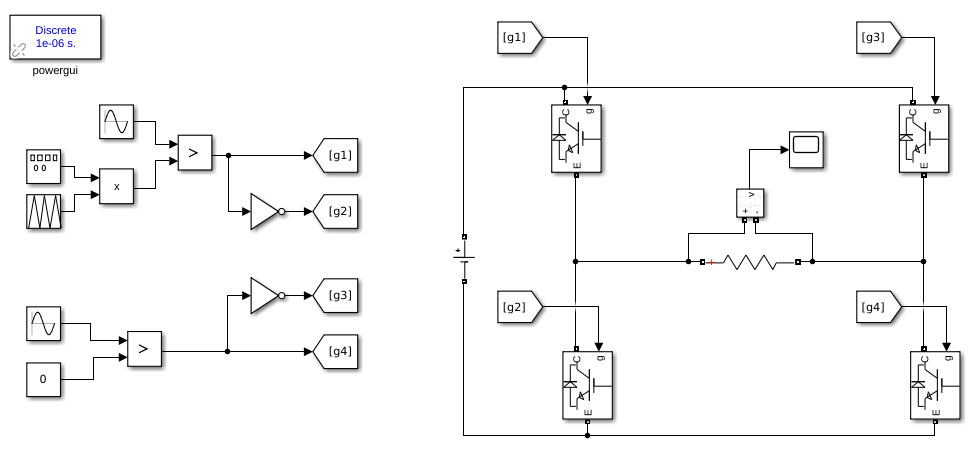
\includegraphics[width=0.9\linewidth,height=\textheight,keepaspectratio]{images/unipolar_modulation_model.png}

}

\caption{\label{fig-model-no-lf}Simulink model with resistive load and
no filter inductor (right side). Gate signals g1--g4 are generated by
the unipolar SPWM subsystem (left side). The voltage measurement block
probes \(V_{ab}\) directly.}

\end{figure}%

\subsection*{\texorpdfstring{With Filter Inductor (\(L_f\) in
circuit)}{With Filter Inductor (L\_f in circuit)}}\label{sec-model-with-lf}
\addcontentsline{toc}{subsection}{With Filter Inductor (\(L_f\) in
circuit)}

The filter inductor \(L_f\) is connected in series to the resistive
load. The voltage scope is placed to measure the waveform output of the
actual load voltage after filtering.

\begin{figure}

\centering{

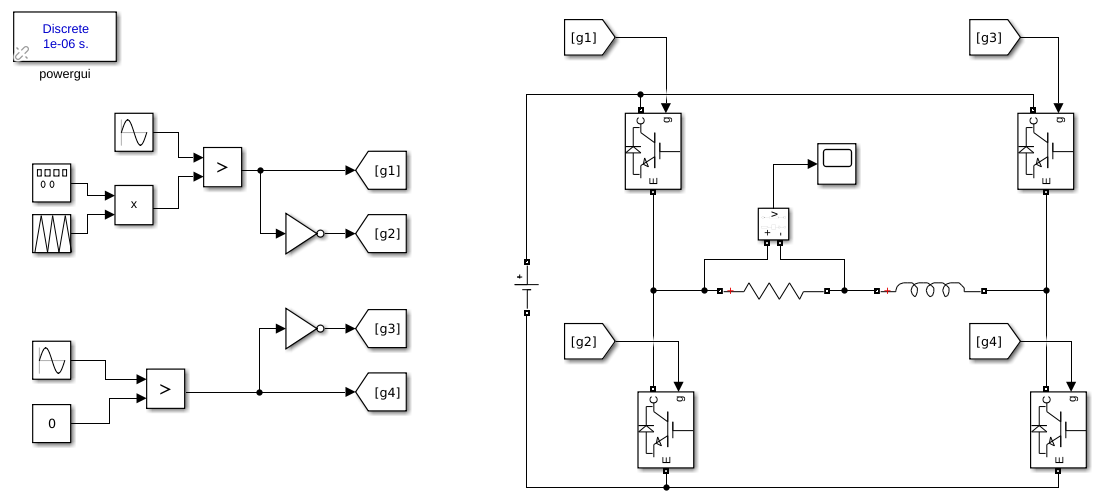
\includegraphics[width=0.9\linewidth,height=\textheight,keepaspectratio]{images/unipolar_modulation_filtered_model.png}

}

\caption{\label{fig-model-with-lf}Simulink model with filter inductor
\(L_f\) added in series with the resistive load. The voltage scope is
tapped across \(R\) only.}

\end{figure}%

\section*{Output Voltage Waveform and FFT
Analysis}\label{sec-output-voltage}
\addcontentsline{toc}{section}{Output Voltage Waveform and FFT Analysis}

\markright{Output Voltage Waveform and FFT Analysis}

\subsection*{Without Filter Inductor}\label{sec-fft-no-lf}
\addcontentsline{toc}{subsection}{Without Filter Inductor}

Without \(L_f\), the bridge output voltage \(V_{ab}\) is a three-level
switching waveform.

\begin{figure}

\centering{

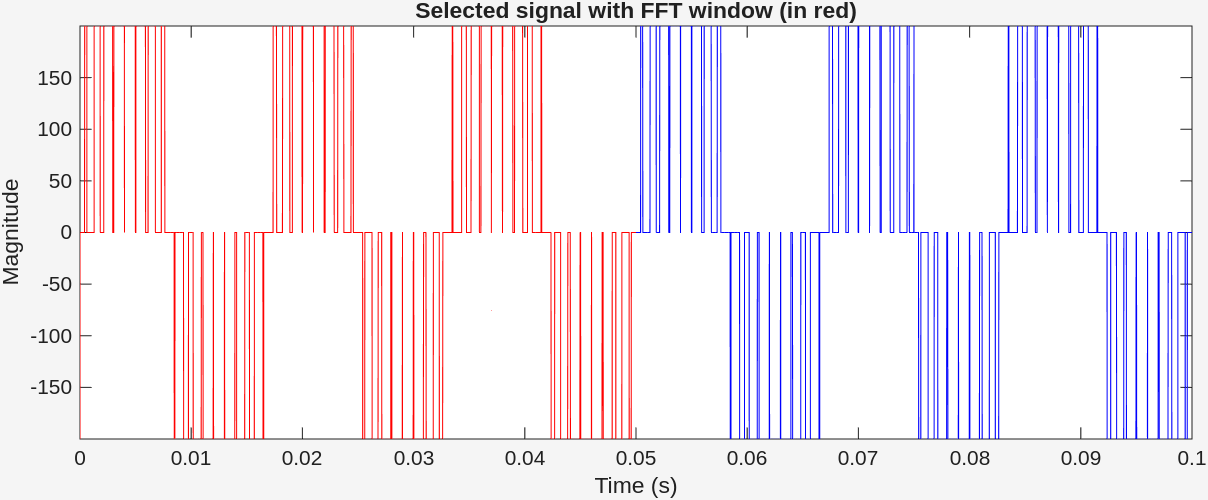
\includegraphics[width=0.9\linewidth,height=\textheight,keepaspectratio]{images/unipolar_modulation_wave.png}

}

\caption{\label{fig-vab-waveform}Time-domain waveform of \(V_{ab}\)
without the filter inductor, showing the characteristic three-level
unipolar switching pattern.}

\end{figure}%

The FFT analysis shows dominant harmonics at 60 Hz and
\(1000 \pm 60\;\mathrm{Hz}\). The THD level is approximately 52.3\%, a
relatively high value due to the presence of low-order harmonics.

\begin{figure}

\centering{

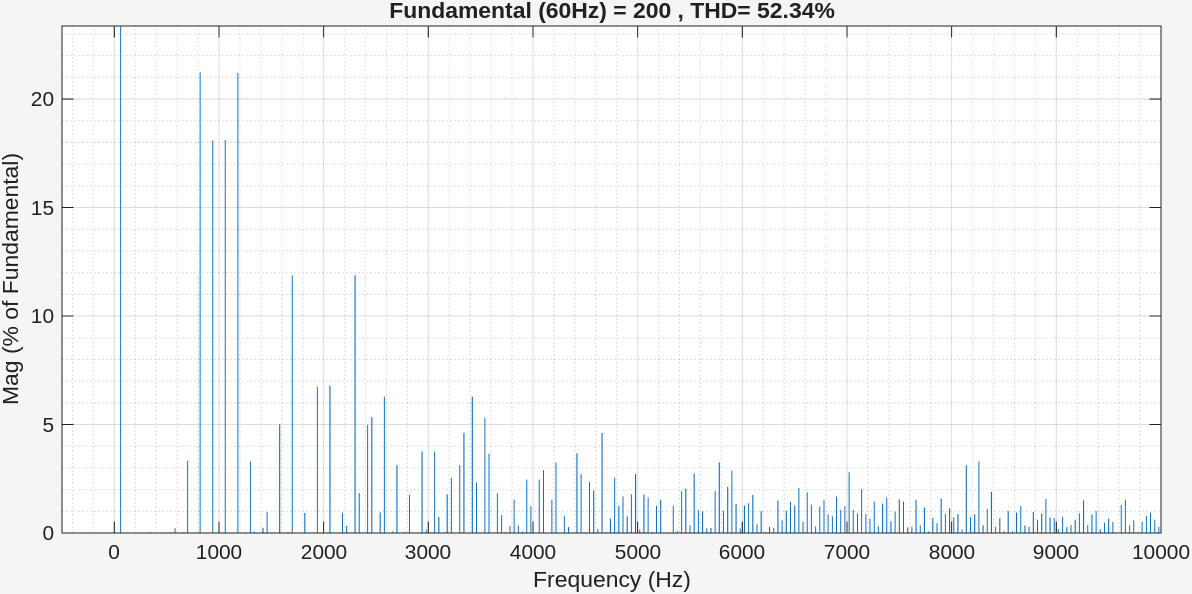
\includegraphics[width=0.9\linewidth,height=\textheight,keepaspectratio]{images/unipolar_modulation_fft.png}

}

\caption{\label{fig-fft-no-lf}FFT spectrum of \(V_{ab}\) (no filter),
obtained from the Simulink Powergui FFT Analysis tool. The fundamental
appears at \(f_1\) and the first significant harmonic cluster appears
near \(2f_{sw}\).}

\end{figure}%

\subsection*{With Filter Inductor}\label{sec-fft-with-lf}
\addcontentsline{toc}{subsection}{With Filter Inductor}

With \(L_f\) reconnected, the inductor acts as a low-pass filter and
attenuates the high-frequency harmonic content. The load voltage across
\(R\) approaches a sinusoidal waveform.

\begin{figure}

\centering{

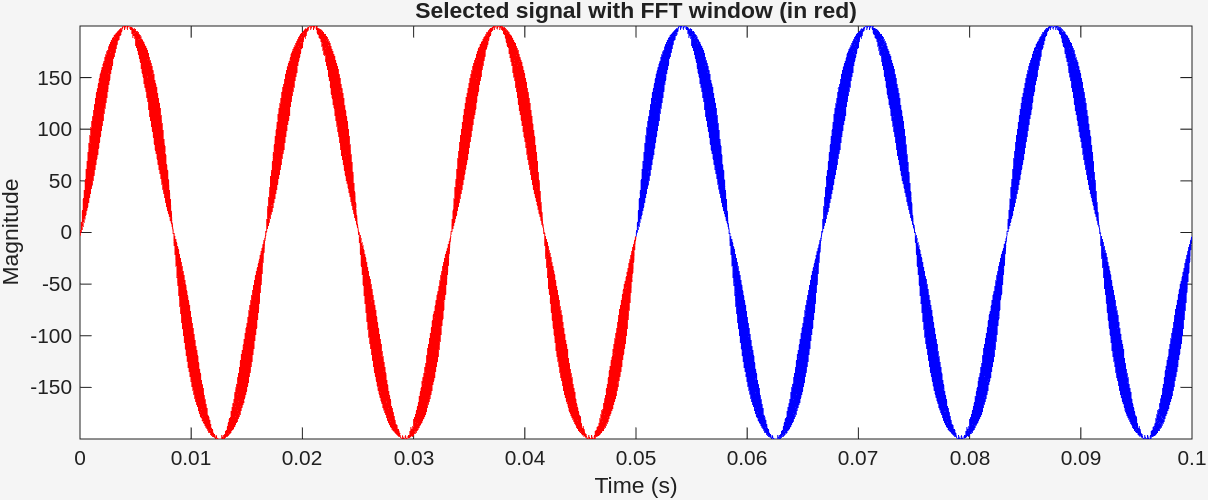
\includegraphics[width=0.9\linewidth,height=\textheight,keepaspectratio]{images/unipolar_modulation_filtered_wave.png}

}

\caption{\label{fig-vload-waveform}Voltage waveform across the resistive
load with \(L_f\) in circuit. The waveform is substantially more
sinusoidal than \(V_{ab}\) without the filter.}

\end{figure}%

The FFT analysis confirms that the dominant harmonic content has been
shifted to higher frequencies, with the THD reduced to a much lower
value of about 9\%, indicating effective filtering.

\begin{figure}

\centering{

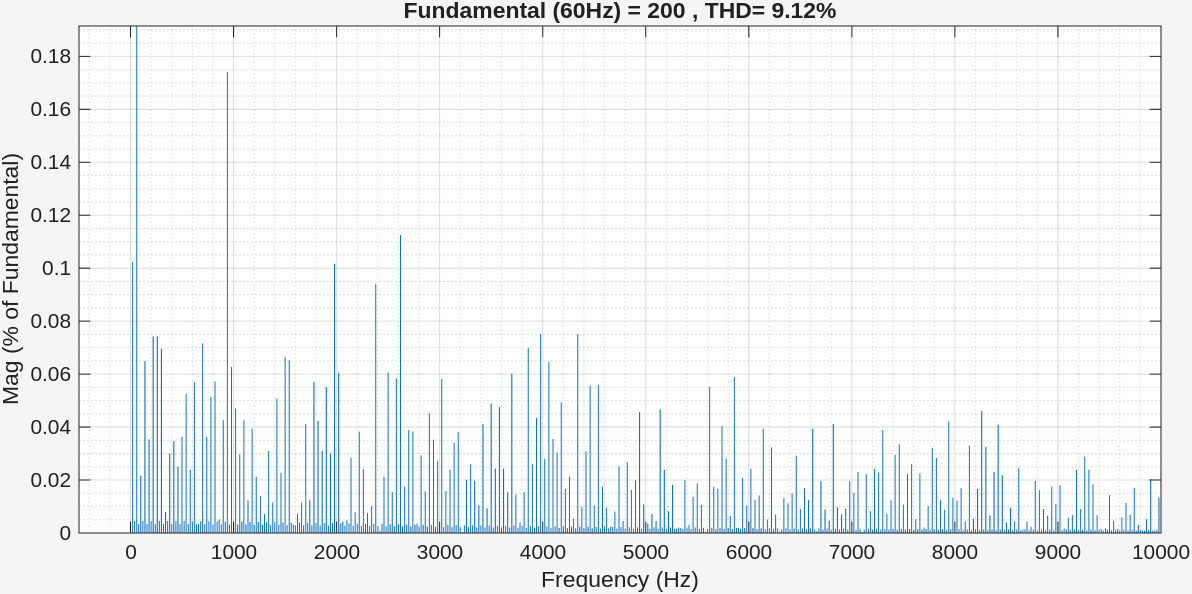
\includegraphics[width=0.9\linewidth,height=\textheight,keepaspectratio]{images/unipolar_modulation_filtered_fft.png}

}

\caption{\label{fig-fft-with-lf}FFT / THD analysis of the load voltage
with \(L_f\), from the Simulink Powergui FFT Analysis tool.}

\end{figure}%

\section*{Comparison with Square Wave Modulation}\label{sec-square-wave}
\addcontentsline{toc}{section}{Comparison with Square Wave Modulation}

\markright{Comparison with Square Wave Modulation}

To benchmark harmonic performance, the gate-signal generator was
replaced with a simple square-wave source operating at the fundamental
frequency \(f_1\). In this scheme, S1 and S4 conduct simultaneously
during the positive half-cycle while S2 and S3 conduct during the
negative half-cycle, producing a two-level output (\(+V_{dc}\) /
\(-V_{dc}\)) with no carrier modulation, as shown in
Figure~\ref{fig-model-sq} on the left side.

\begin{figure}

\centering{

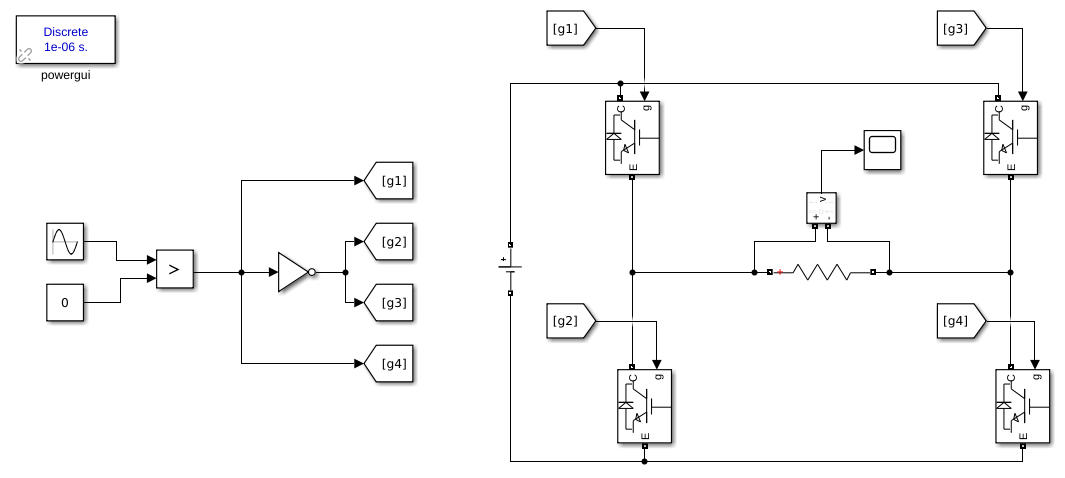
\includegraphics[width=0.9\linewidth,height=\textheight,keepaspectratio]{images/square_modulation_model.png}

}

\caption{\label{fig-model-sq}Time-domain waveform of \(V_{ab}\) under
square-wave switching, showing the characteristic two-level pattern.}

\end{figure}%

The output voltage waveform is a simple square wave, and the FFT
spectrum shows significant low-order harmonic content, with the
harmonics of 60 Hz, 180 Hz, 300 Hz, etc., corresponding to 1st, 3rd,
5th, etc. harmonics of the fundamental frequency. The THD is
approximately 48.3\%, which is higher than that of unipolar SPWM with
filtering.

\begin{figure}

\centering{

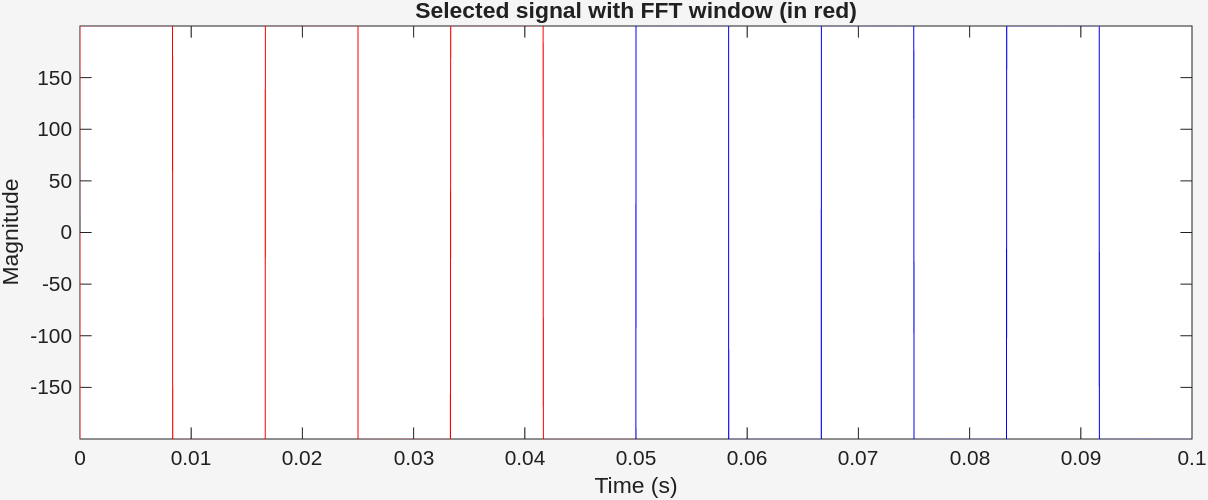
\includegraphics[width=0.9\linewidth,height=\textheight,keepaspectratio]{images/square_modulation_wave.png}

}

\caption{\label{fig-vab-sq}Voltage waveform across the resistive load
under square-wave switching. The waveform is a simple two-level square
wave, with significant low-order harmonic content.}

\end{figure}%

\begin{figure}

\centering{

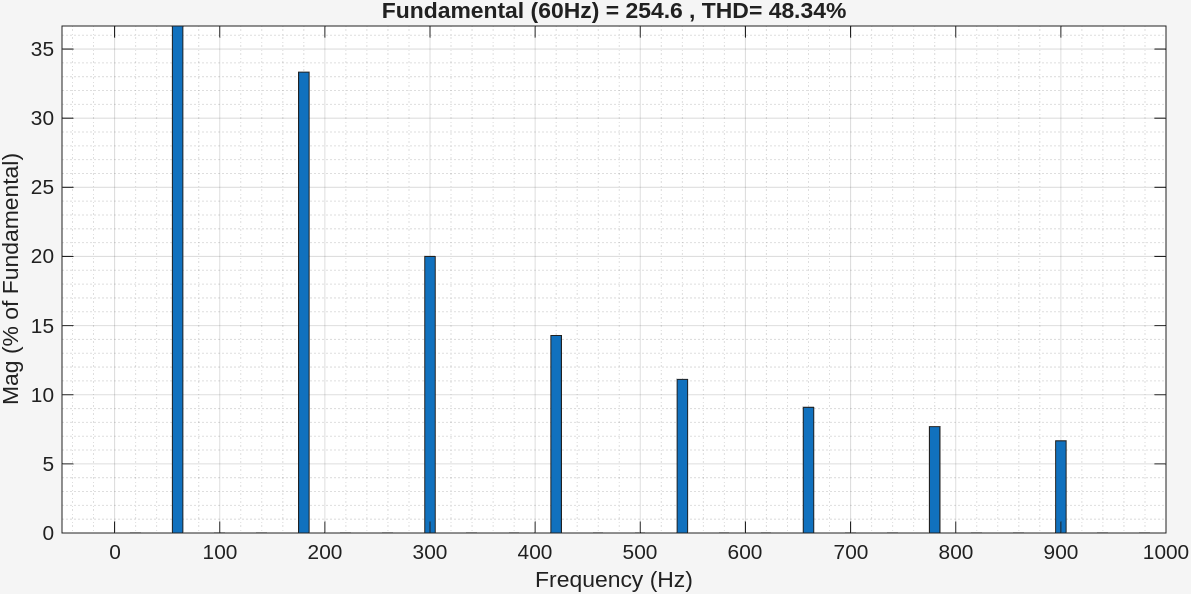
\includegraphics[width=0.9\linewidth,height=\textheight,keepaspectratio]{images/square_modulation_fft.png}

}

\caption{\label{fig-fft-sq}FFT spectrum of \(V_{ab}\) under square-wave
switching, overlaid with the unipolar SPWM spectrum for direct
comparison.}

\end{figure}%

\section*{Simulink Model --- Grid-Connected
Operation}\label{sec-grid-model}
\addcontentsline{toc}{section}{Simulink Model --- Grid-Connected
Operation}

\markright{Simulink Model --- Grid-Connected Operation}

In the grid-connected configuration the resistive load is replaced by an
AC grid voltage source \(V_g\) connected through the filter inductor
\(L_f\). The inverter must synthesise an output voltage \(V_{ab}\) whose
amplitude and phase are determined by the grid voltage and the desired
injected current.

\subsection*{Steady-State Phasor Analysis}\label{sec-phasor}
\addcontentsline{toc}{subsection}{Steady-State Phasor Analysis}

\begin{figure}

\centering{

\pandocbounded{\includegraphics[keepaspectratio]{index_files/mediabag/046d2aa7f2009f11e171720822779f3671ec9208.pdf}}

}

\caption{\label{fig-circuit-grid}Circuit diagram of the grid-connected
inverter with filter inductor \(L_f\) and grid voltage source \(V_g\).
The inverter output voltage \(V_{ab}\) is measured across the series
combination of \(L_f\) and \(V_g\).}

\end{figure}%

The KVL equation around the output loop (Figure~\ref{fig-circuit-grid})
gives:

\begin{equation}\phantomsection\label{eq-kvl}{
V_{ab} = V_L + V_g
}\end{equation}

where \(V_L = j\omega I_{L_f} L_f\) is the phasor voltage across the
filter inductor.

\begin{figure}

\centering{

\pandocbounded{\includegraphics[keepaspectratio]{index_files/mediabag/034184bb4852e513f9706ddfc3e631ed7c47cc19.pdf}}

}

\caption{\label{fig-phasor}Phasor diagram showing the relationship
between the grid voltage \(V_g\), the inductor voltage \(V_L\), and the
inverter output voltage \(V_{ab}\). The angle \(\theta\) represents the
phase lead of \(V_{ab}\) over \(V_g\).}

\end{figure}%

With the grid current \(I_{L_f} = 1\angle 0°\;\mathrm{A}\) (amplitude,
taken as the reference phasor) and the circuit parameters in
Table~\ref{tbl-params}, the inductor voltage is:

\begin{equation}\phantomsection\label{eq-vl}{
V_L = j\omega L_f \, I_{L_f}
    = j \underbrace{(120\pi)}_{\omega}
      \times \underbrace{(10 \times 10^{-3})}_{L_f}
      \times 1
    \approx 3.77\angle 90°\;\text{V}
}\end{equation}

The grid voltage phasor (in phase with \(I_{L_f}\) for a resistive grid
equivalent) is:

\begin{equation}\phantomsection\label{eq-vg}{
V_g = 120\sqrt{2} \approx 169.68\angle 0°\;\text{V}
}\end{equation}

Because \(V_L \perp V_g\) in the phasor diagram
(Figure~\ref{fig-phasor}), the required inverter output amplitude is:

\begin{equation}\phantomsection\label{eq-vab-mag}{
V_{ab} = \sqrt{V_L^2 + V_g^2}
         = \sqrt{3.77^2 + 169.68^2}
         = \sqrt{14.21 + 28\,791.38}
         \approx 169.722\;\text{V}
}\end{equation}

The corresponding phase lead of \(V_{ab}\) over \(V_g\) is:

\begin{equation}\phantomsection\label{eq-theta}{
\theta = \arctan\!\left(\frac{V_L}{V_g}\right)
       = \arctan\!\left(\frac{3.77}{169.68}\right)
       \approx 0.0222\;\text{rad}
       \equiv 1.2728°
}\end{equation}

Finally, the modulation index required to produce this output from a
\(V_{dc} = 200\;\text{V}\) DC bus is:

\begin{equation}\phantomsection\label{eq-ma}{
\boxed{m_a = \frac{|V_{ab}|}{V_{dc}}
           = \frac{169.722}{200}
           \approx 0.84861}
}\end{equation}

\subsection*{Simulink Model Screenshots}\label{sec-grid-screenshots}
\addcontentsline{toc}{subsection}{Simulink Model Screenshots}

The sinusoidal reference amplitude and phase offset were set in the
unipolar SPWM subsystem (top-left in Figure~\ref{fig-grid-model}) to
match the phasor analysis results in \textbf{?@sec-phasor}. The current
measurement block was placed in series with \(L_f\) to probe the grid
current waveform.

\begin{figure}

\centering{

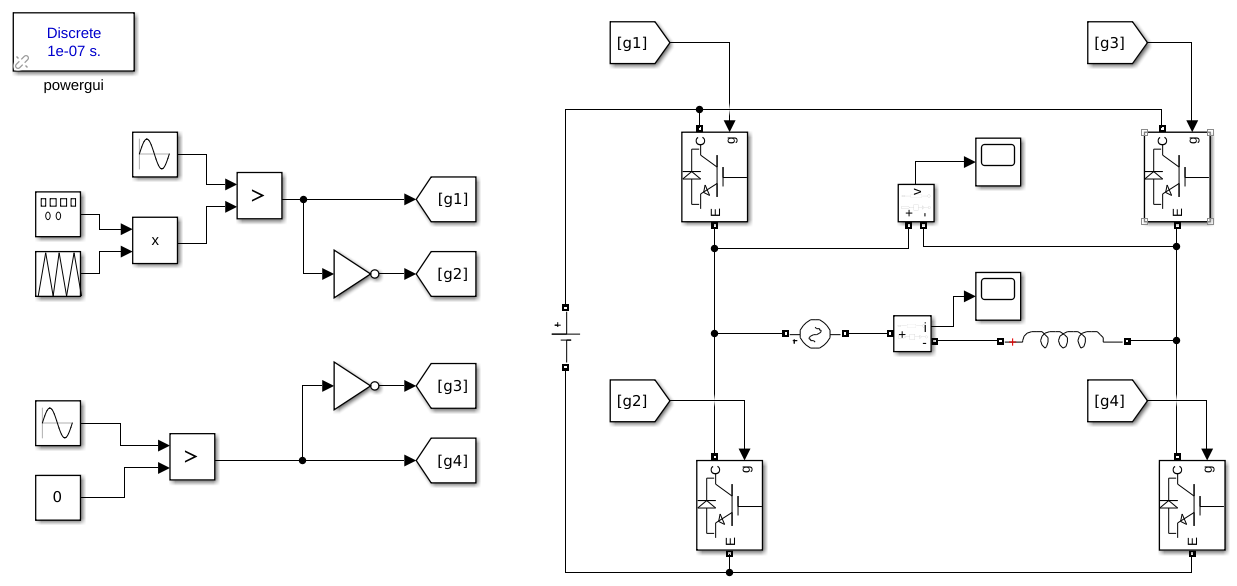
\includegraphics[width=0.9\linewidth,height=\textheight,keepaspectratio]{images/unipolar_modulation_grid_operation_model.png}

}

\caption{\label{fig-grid-model}Top-level Simulink model for
grid-connected operation. The series path from the bridge output is:
\(L_f\) → current measurement block → AC voltage source \(V_g\). The
current scope is a series ammeter block, not a parallel voltage
measurement.}

\end{figure}%

Waveforms were captured from the current scope, showing the grid current
\(i_g(t)\) in phase with the grid voltage \(V_g\) for unity power-factor
injection. The THD of the grid current was measured to be approximately
13\%, indicating that the inverter is effectively injecting a nearly
sinusoidal current into the grid.

\begin{figure}

\centering{

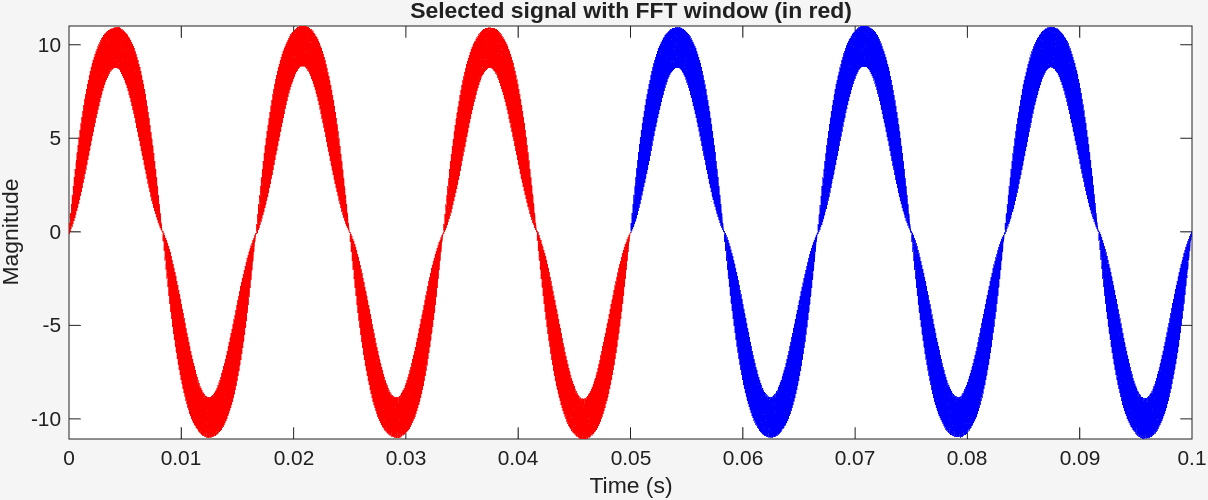
\includegraphics[width=0.9\linewidth,height=\textheight,keepaspectratio]{images/unipolar_modulation_grid_operation_wave.png}

}

\caption{\label{fig-grid-current}Grid current waveform \(i_g(t)\) (in
Amphere) with \(L_f\) in circuit. The waveform is approximately
sinusoidal and in phase with \(V_g\) for unity power-factor injection.}

\end{figure}%

\begin{figure}

\centering{

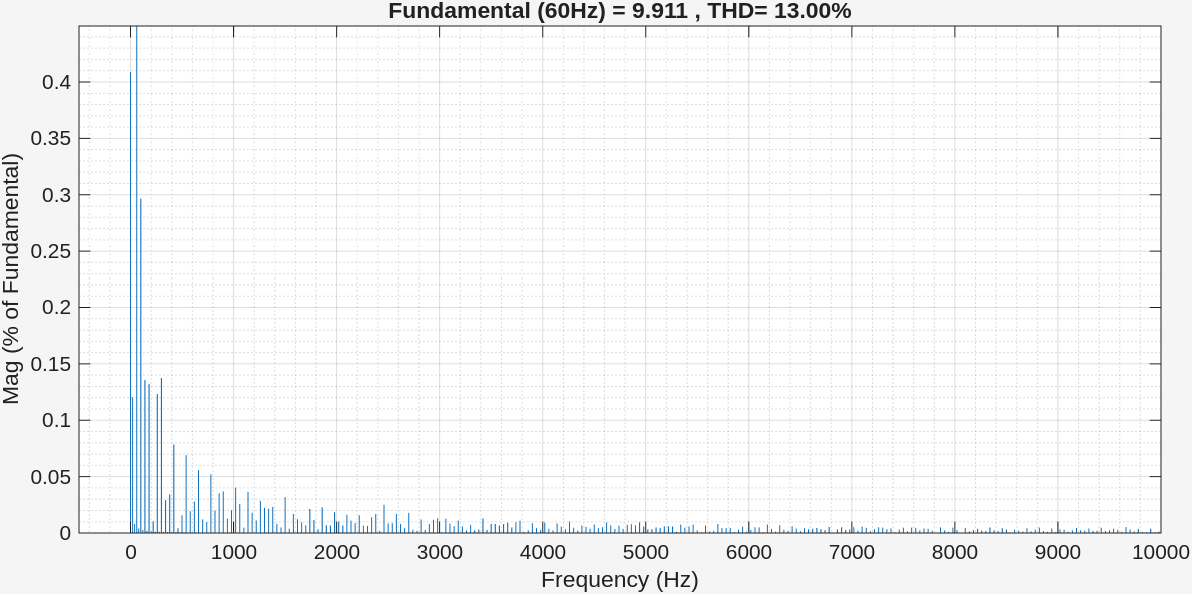
\includegraphics[width=0.9\linewidth,height=\textheight,keepaspectratio]{images/unipolar_modulation_grid_operation_fft.png}

}

\caption{\label{fig-fft-igrid}FFT / THD analysis of the grid current
from the Simulink Powergui FFT Analysis tool.}

\end{figure}%

\section*{Conclusion}\label{sec-conclusion}
\addcontentsline{toc}{section}{Conclusion}

\markright{Conclusion}

This report demonstrated the simulation of a single-phase grid-connected
full-bridge inverter using unipolar SPWM in MATLAB/Simulink. The
inverter was first tested with a resistive load, both without and with a
filter inductor \(L_f\). The FFT analysis confirmed that the filter
effectively reduced the THD of the load voltage from 52.3\% to 9\%.
Compared to square-wave switching, unipolar SPWM produced a three-level
output voltage with dominant harmonics shifted to higher frequencies,
producing a unfiltered THD of 48.3\%.

The phasor analysis in \textbf{?@sec-phasor} showed that the inverter
output voltage \(V_{ab}\) must lead the grid voltage \(V_g\) by a small
angle \(\theta \approx 1.2728°\) to drive the desired grid current
\(I_{L_f}\). The required modulation index was calculated to be
approximately \(0.84861\). The Simulink model for grid-connected
operation confirmed that the grid current waveform was approximately
sinusoidal and in phase with the grid voltage, with a THD of about 13\%,
indicating effective harmonic performance.




\end{document}
